%!TEX root = ../Thesis.tex
\chapter{CAD Design}
All tolerances are $1/100$mm, screws and blots are in metric units, dimensions are in mm, and the material is aluminium unless other is stated. 

\subsection{Horizontal angle messurement device}


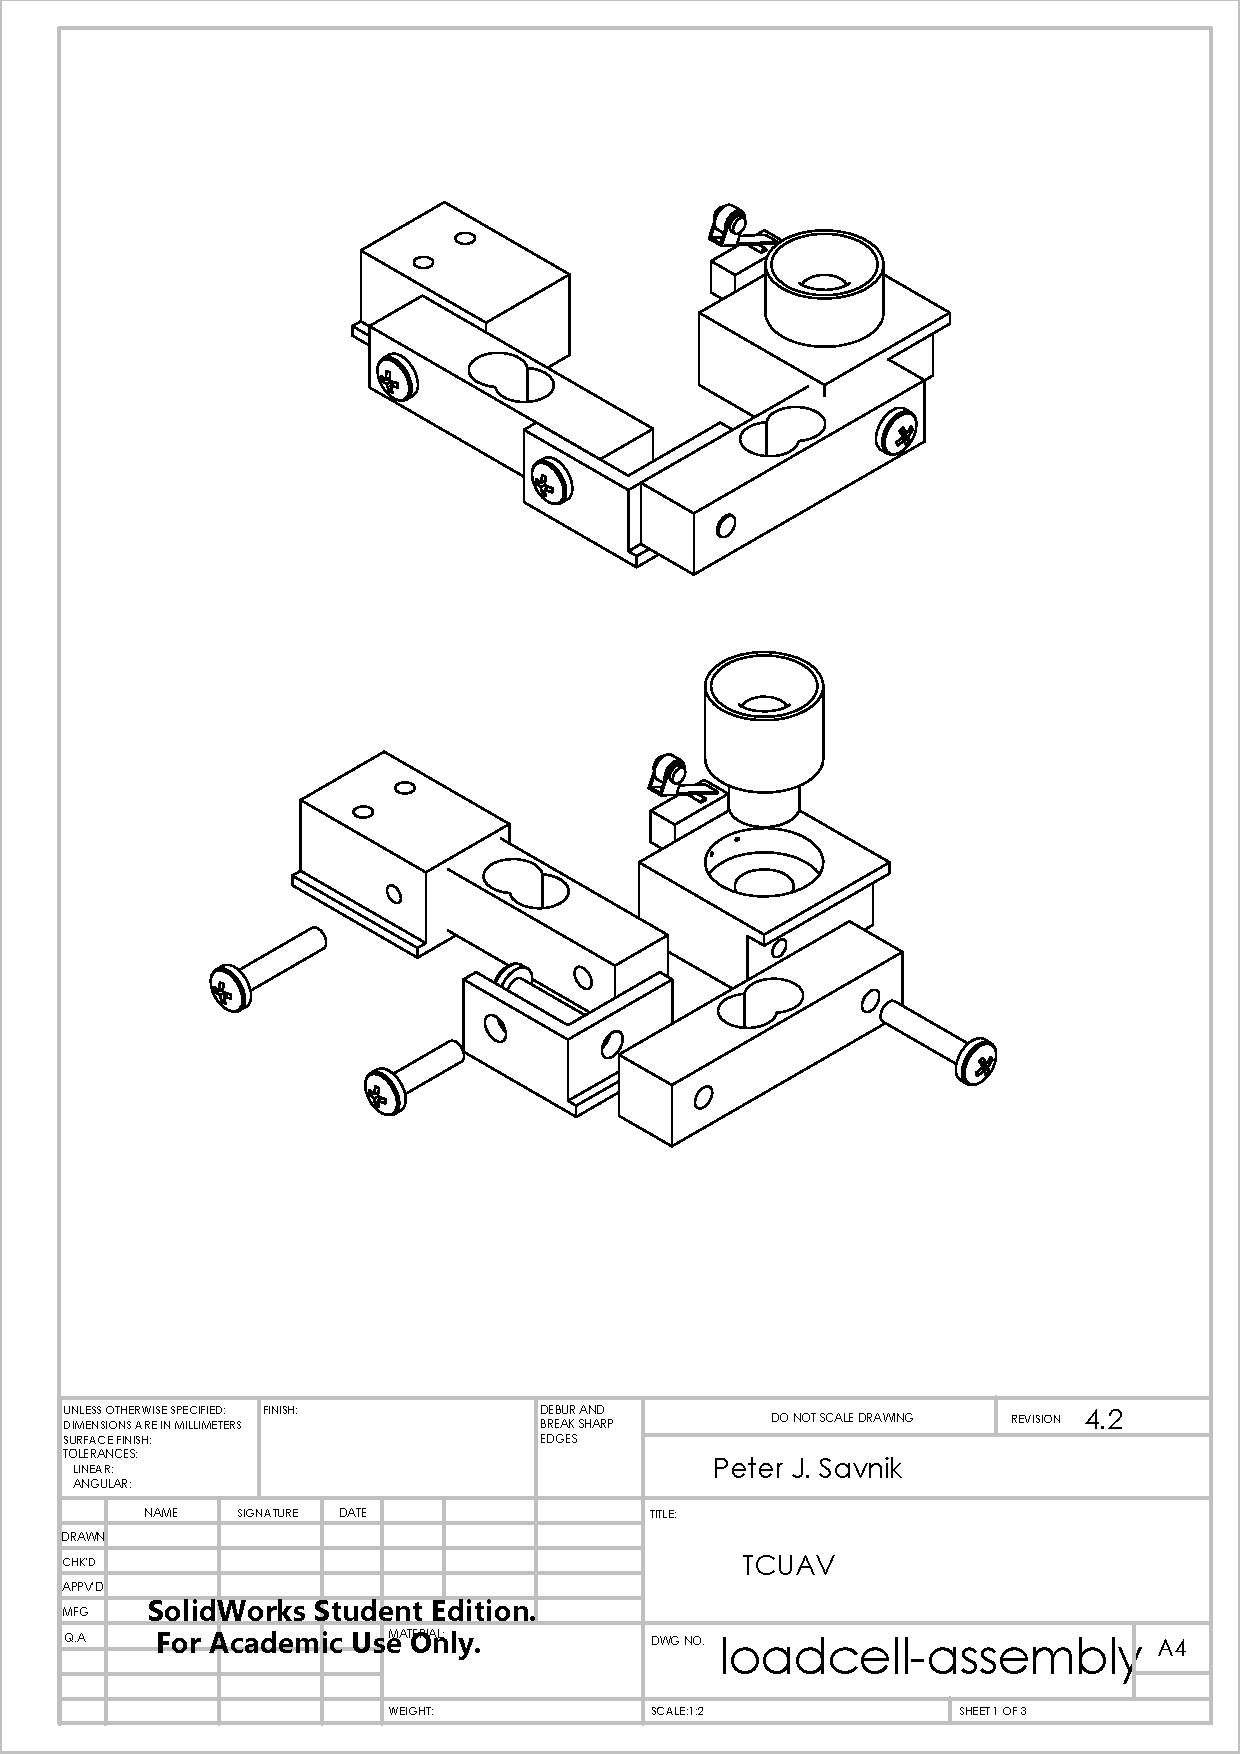
\includepdf[pages={-}]{graphics/cad/loadcell-assembly.pdf}
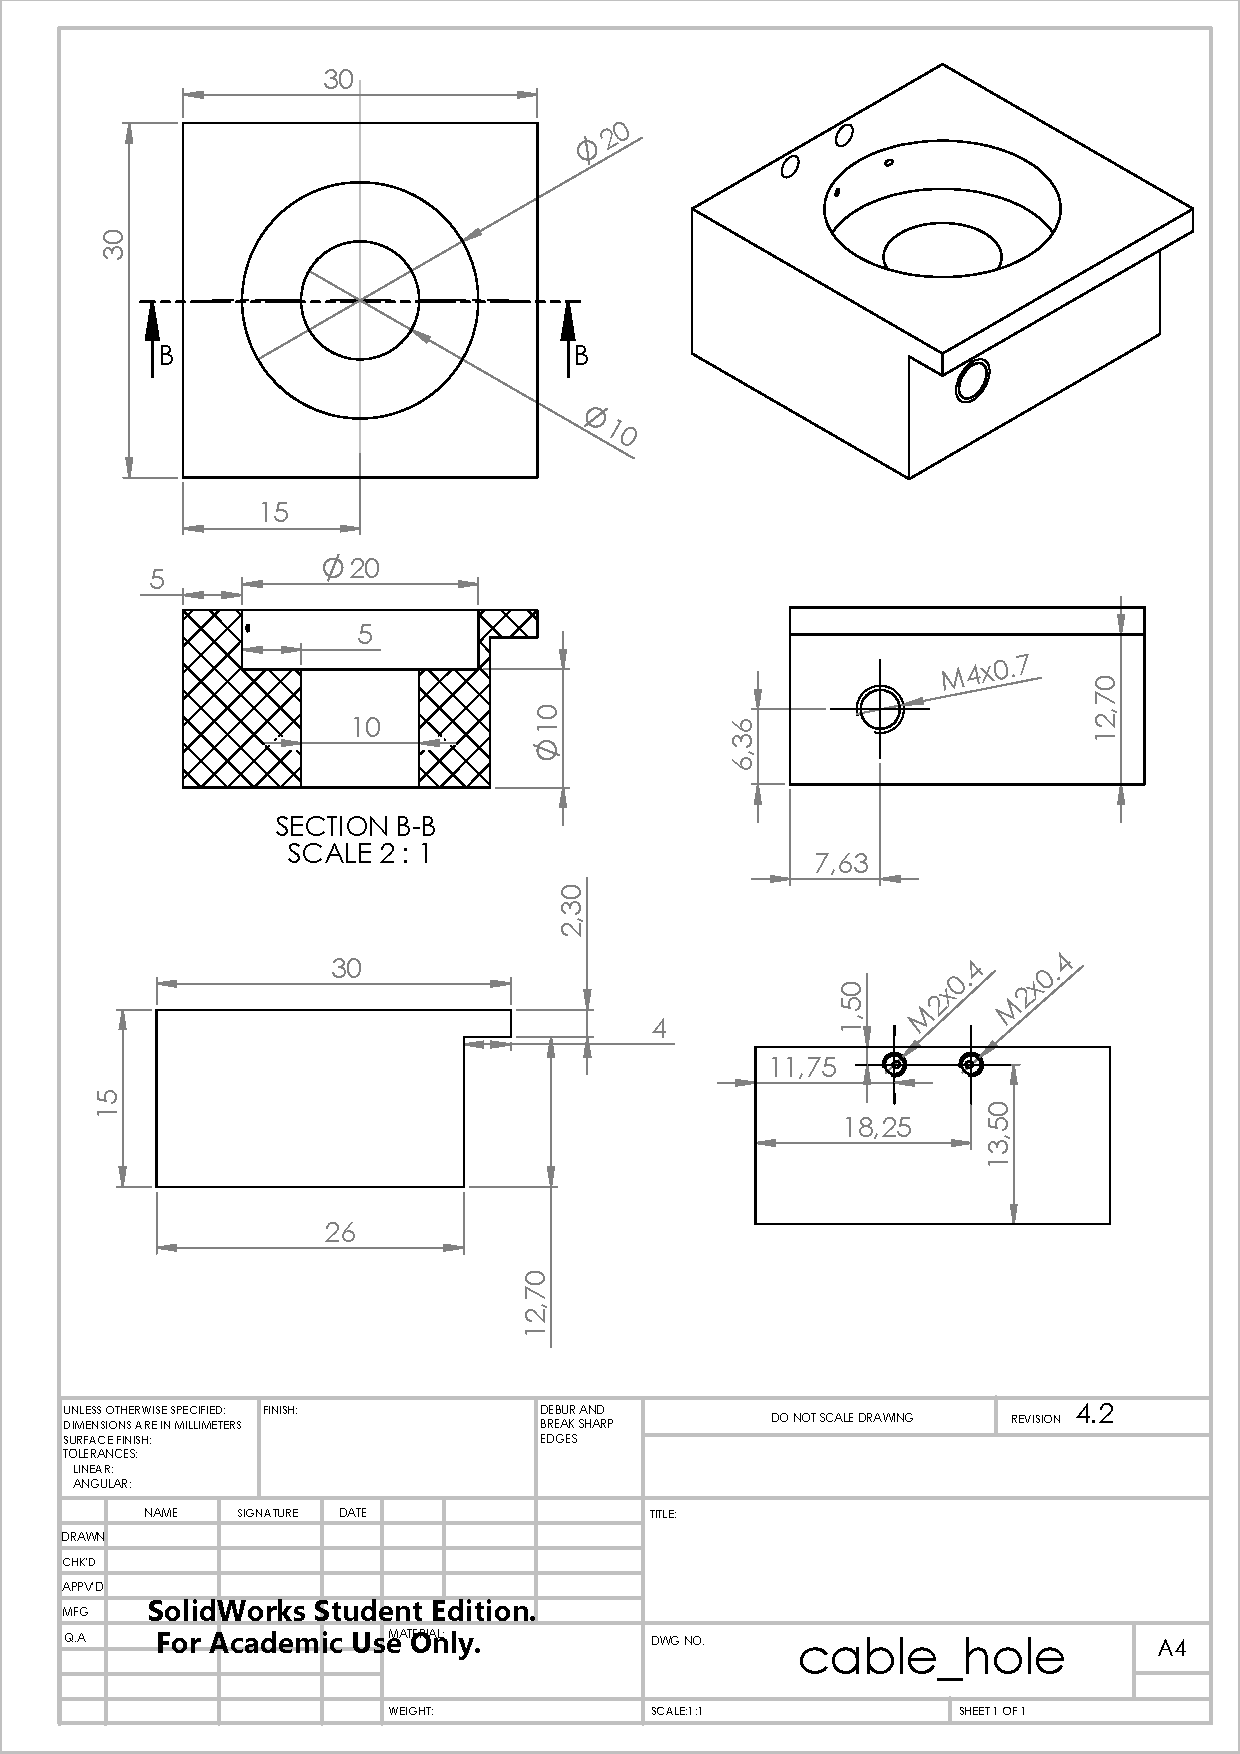
\includepdf[pages={-}]{graphics/cad/cable_hole.pdf}
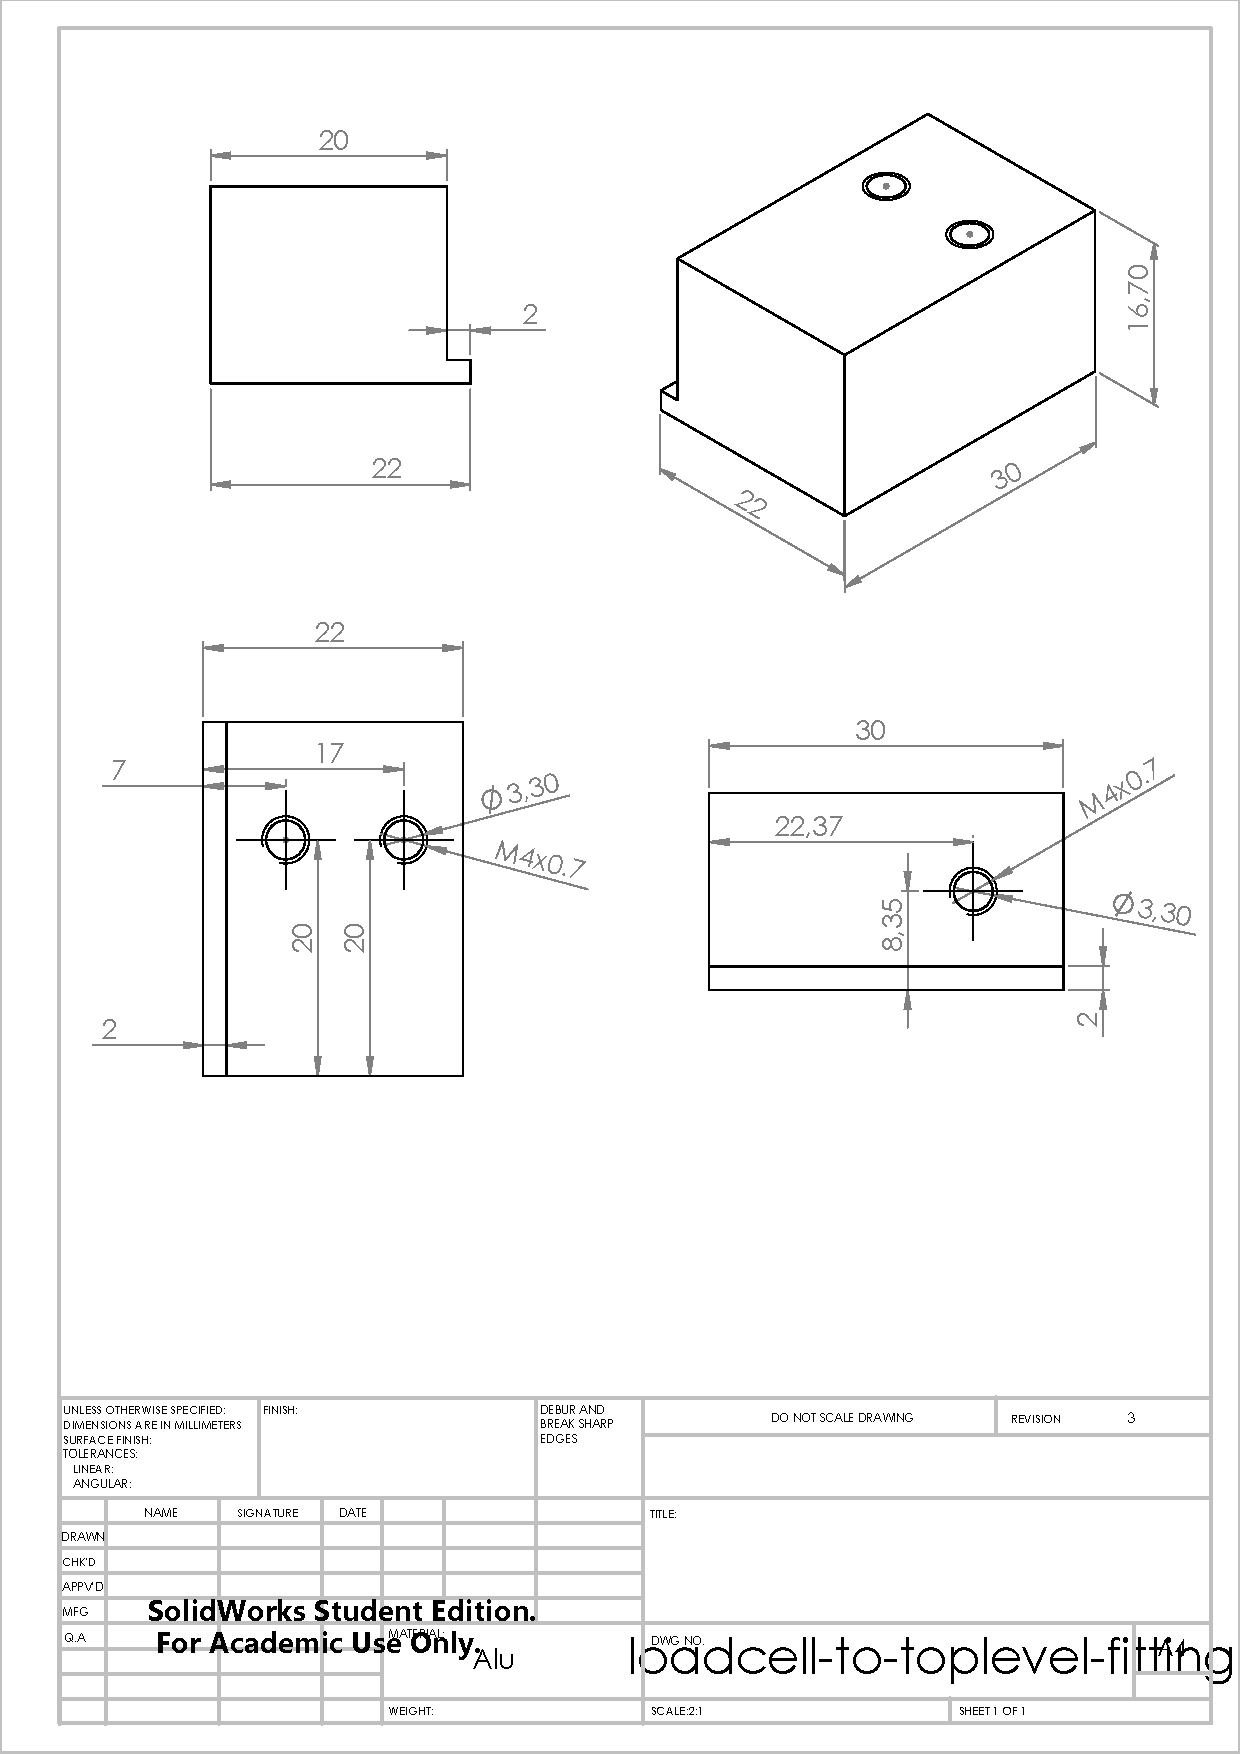
\includepdf[pages={-}]{graphics/cad/loadcell-to-toplevel-fitting.pdf}
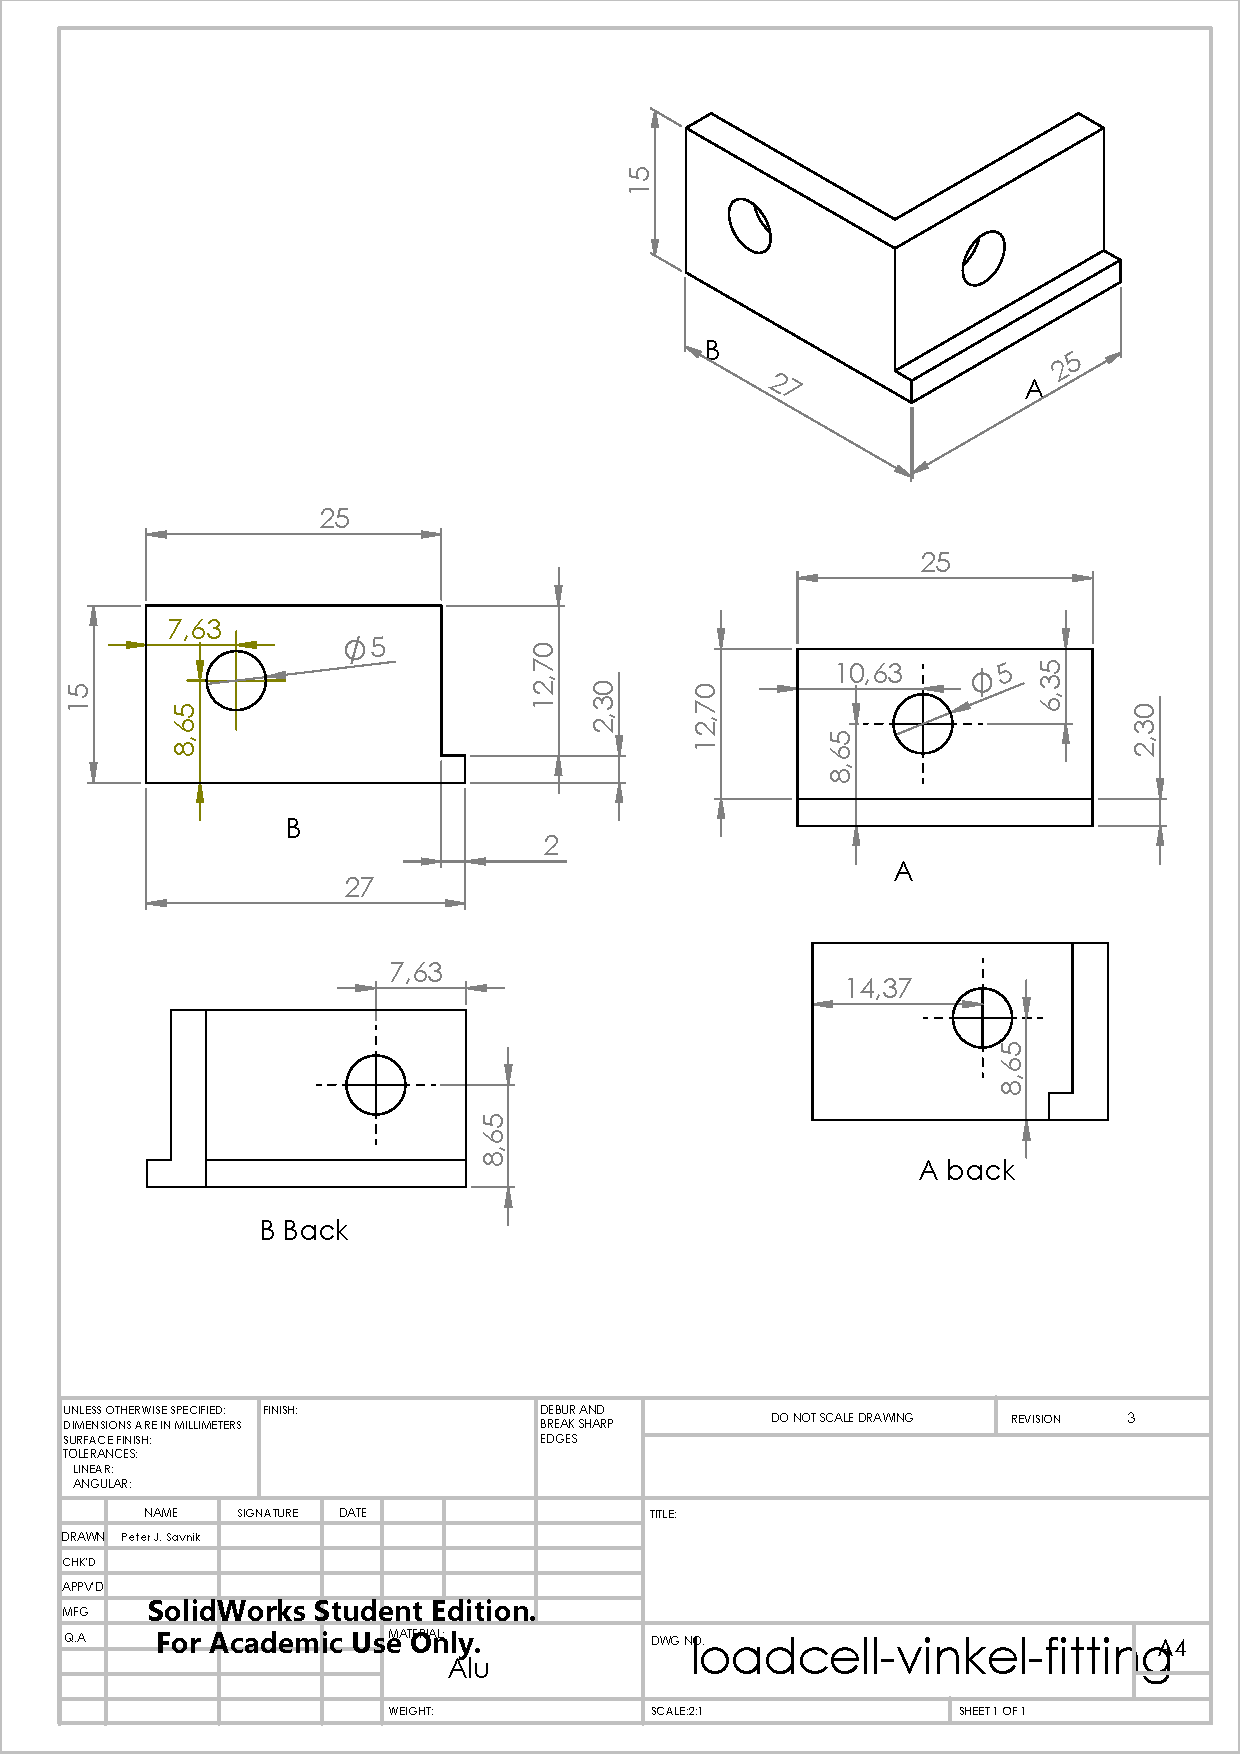
\includepdf[pages={-}]{graphics/cad/loadcell-vinkel-fitting.pdf}
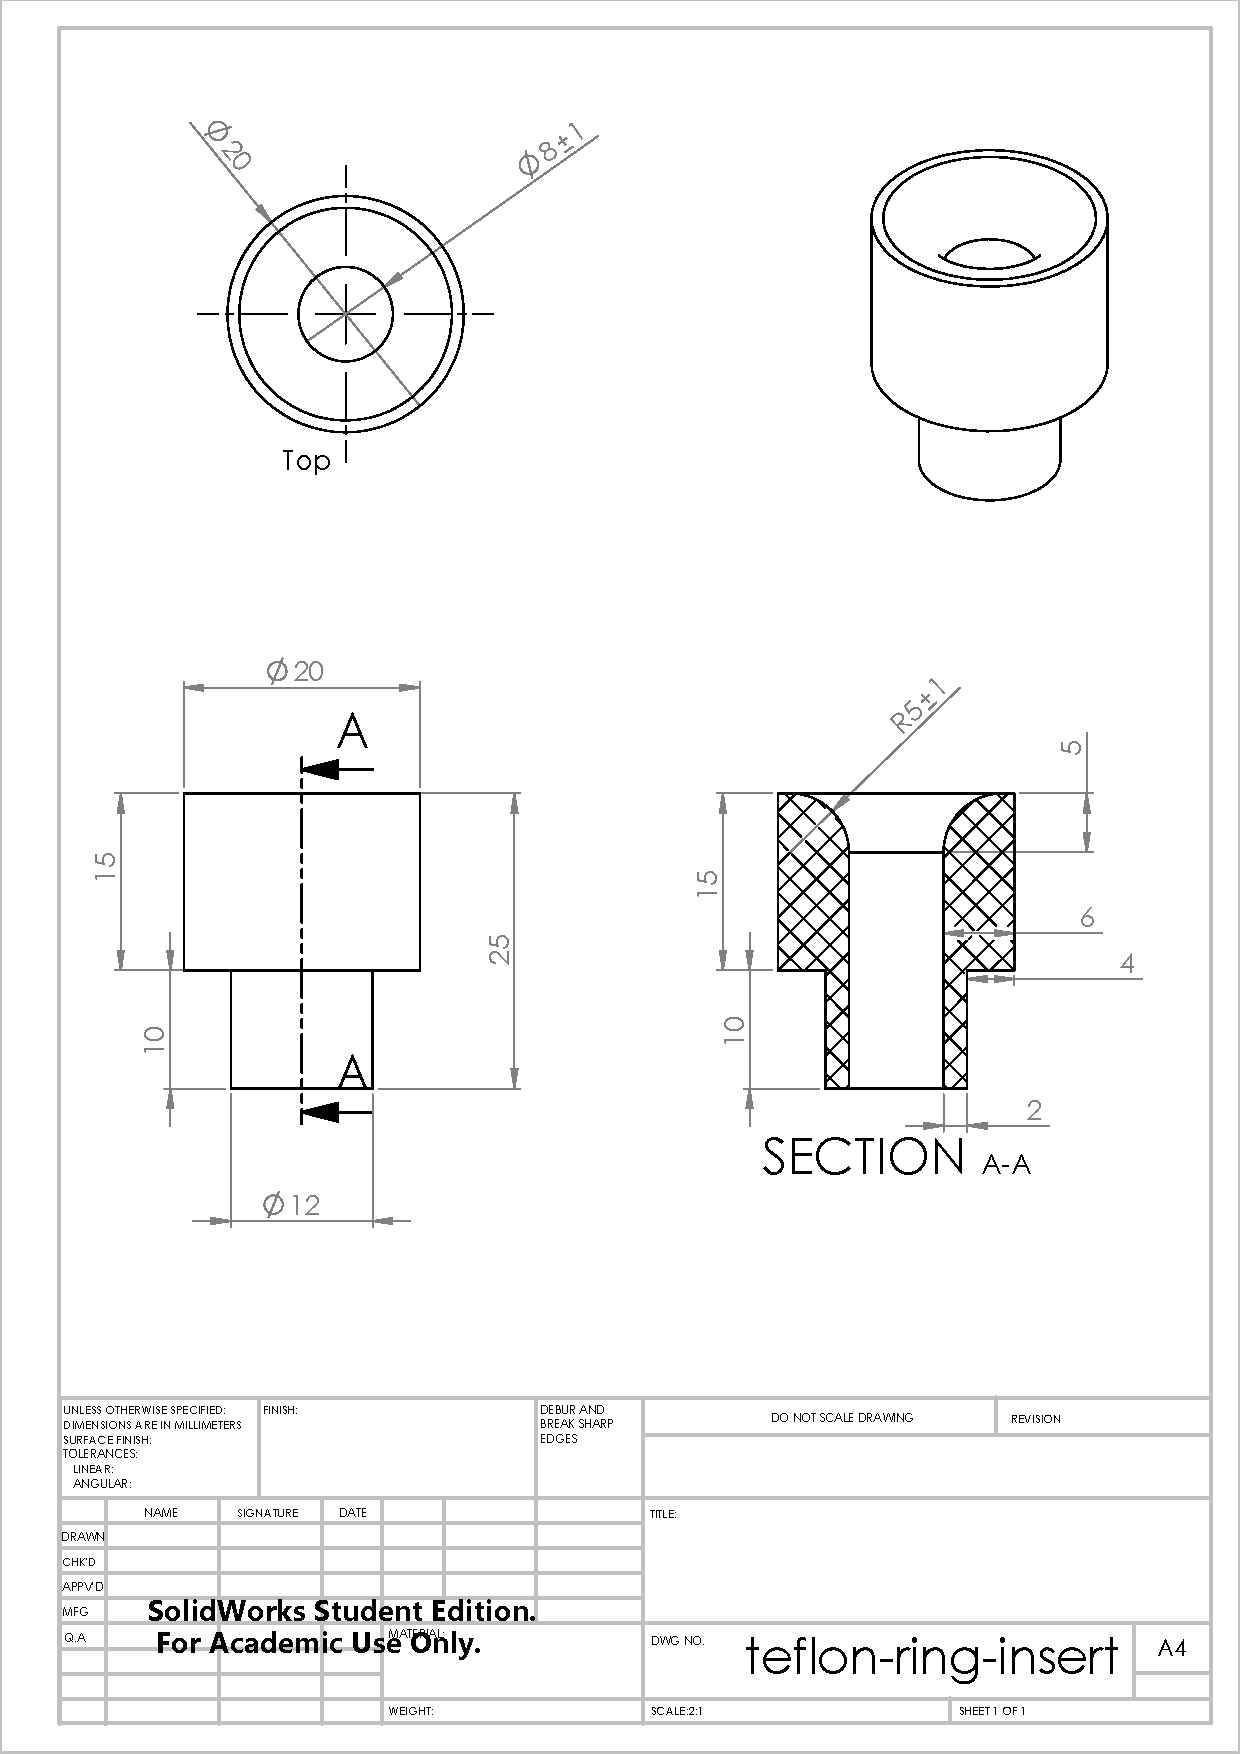
\includepdf[pages={-}]{graphics/cad/teflon-ring-insert.pdf}

\subsection{The Simple Winch}
The simple winch is inspired from 3D printer extruder mechanism. The is pushed between two wheels. One wheel is motorized and fixed in position and second is pushing towards the motor wheel with a spring tension. The spring assures the second wheel always have contact with the cable, even if there is small variations in cable thickness. Second wheel also includes an encoder. Having the encoder on the second wheel, instead of the motor wheel, assures the rotation is actually from the cable and not because the motor wheel slips on the cable. The springs in this prototype is normal ballpoint pen springs taken from two arbitrary ballpoint pens. \\
The encoder is a magnetic encoder with a magnet attached at the end of the shaft. The shaft is made of steel, so the magnet will stick.  
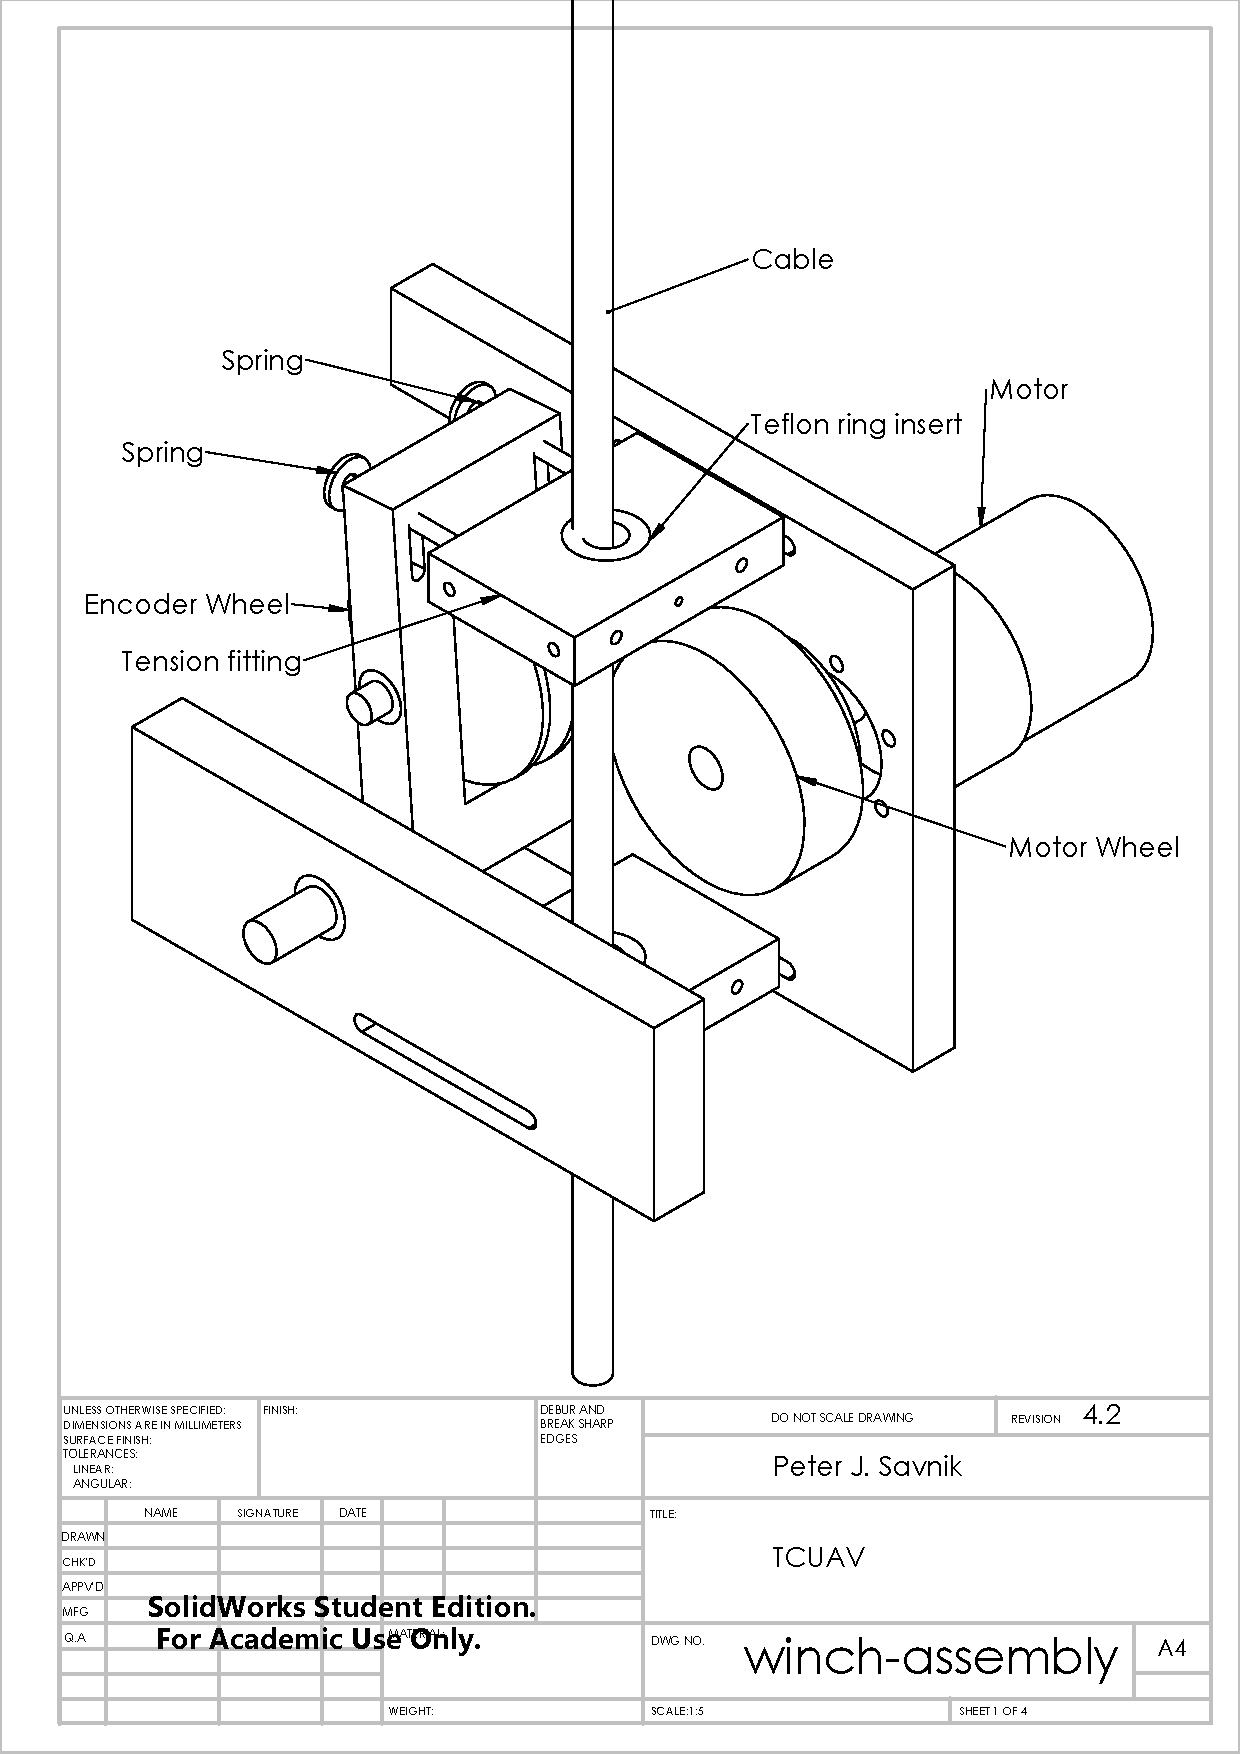
\includepdf[pages={-}]{graphics/cad/winch-assembly.pdf}
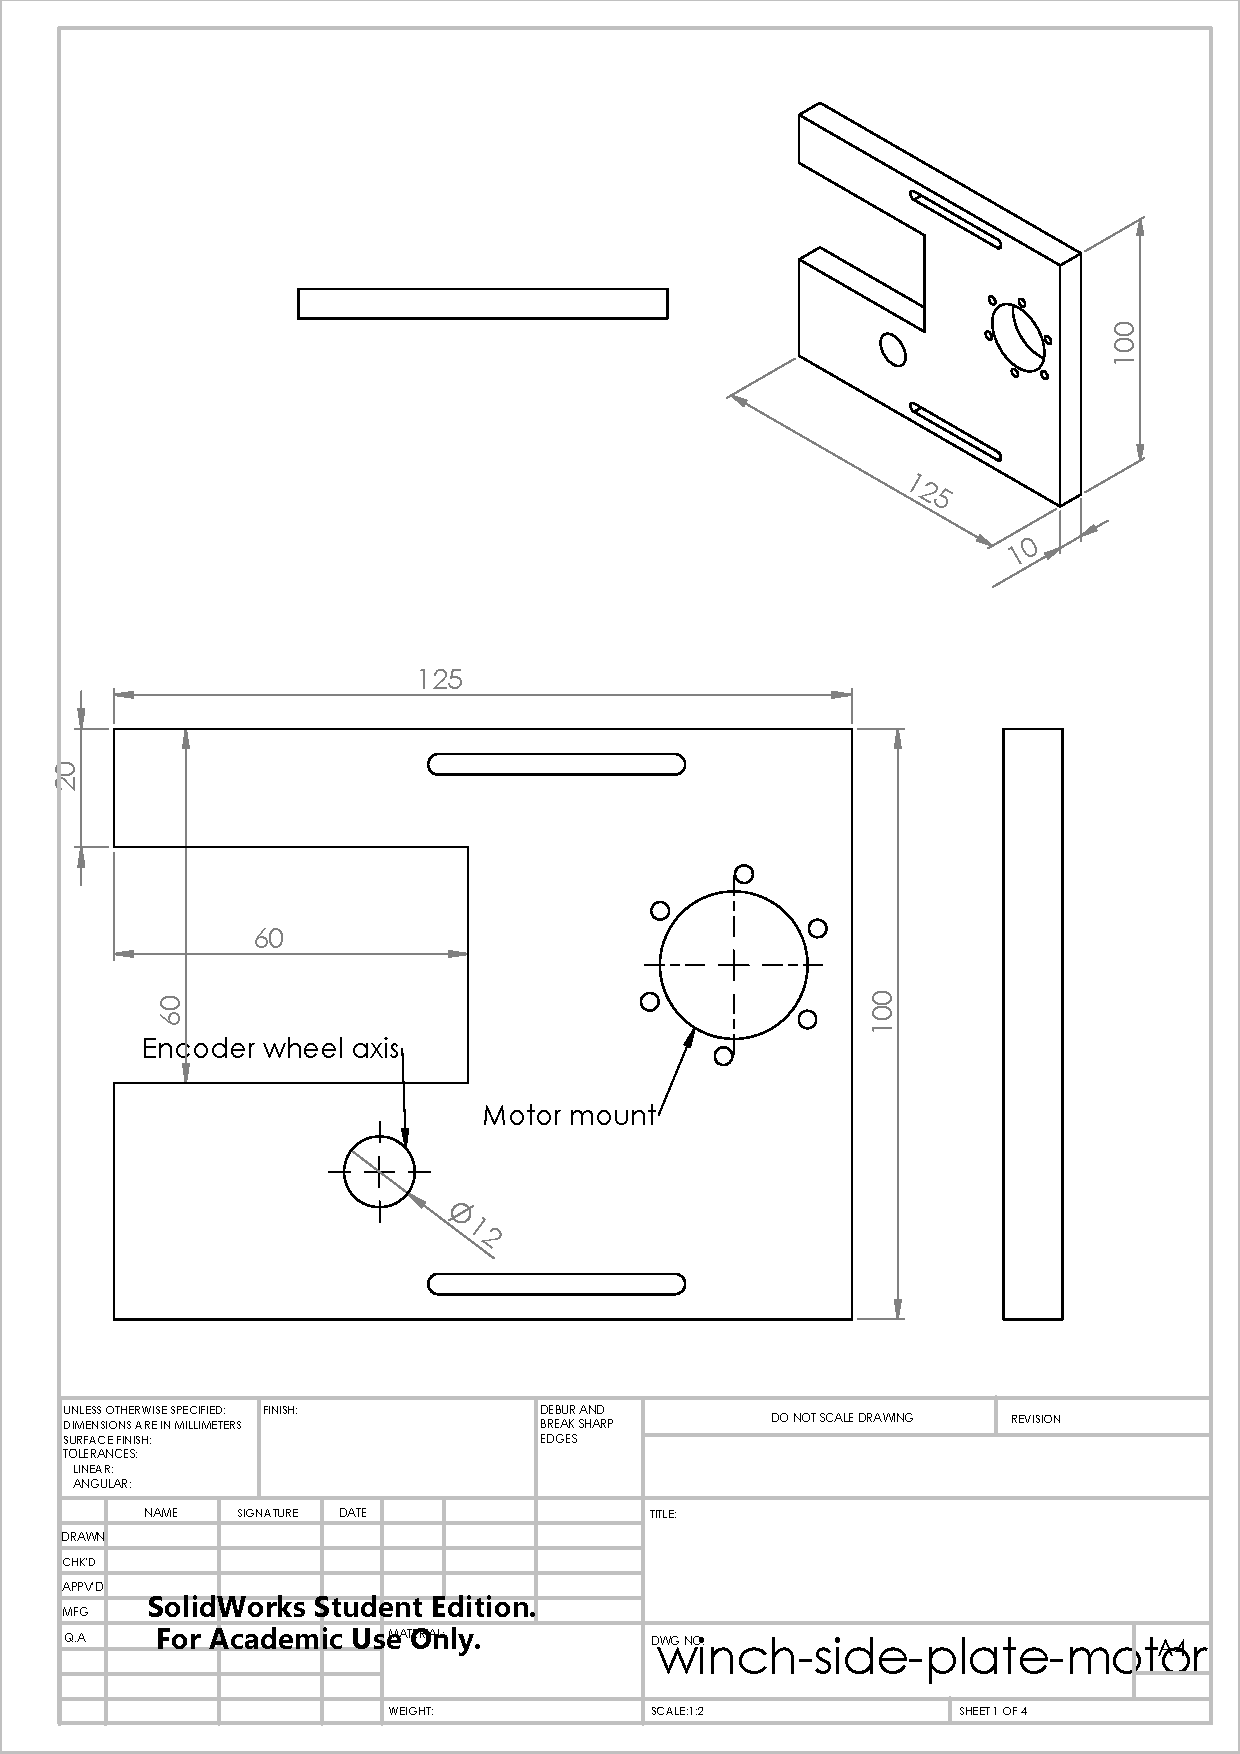
\includepdf[pages={-}]{graphics/cad/winch-side-plate-motor.pdf}
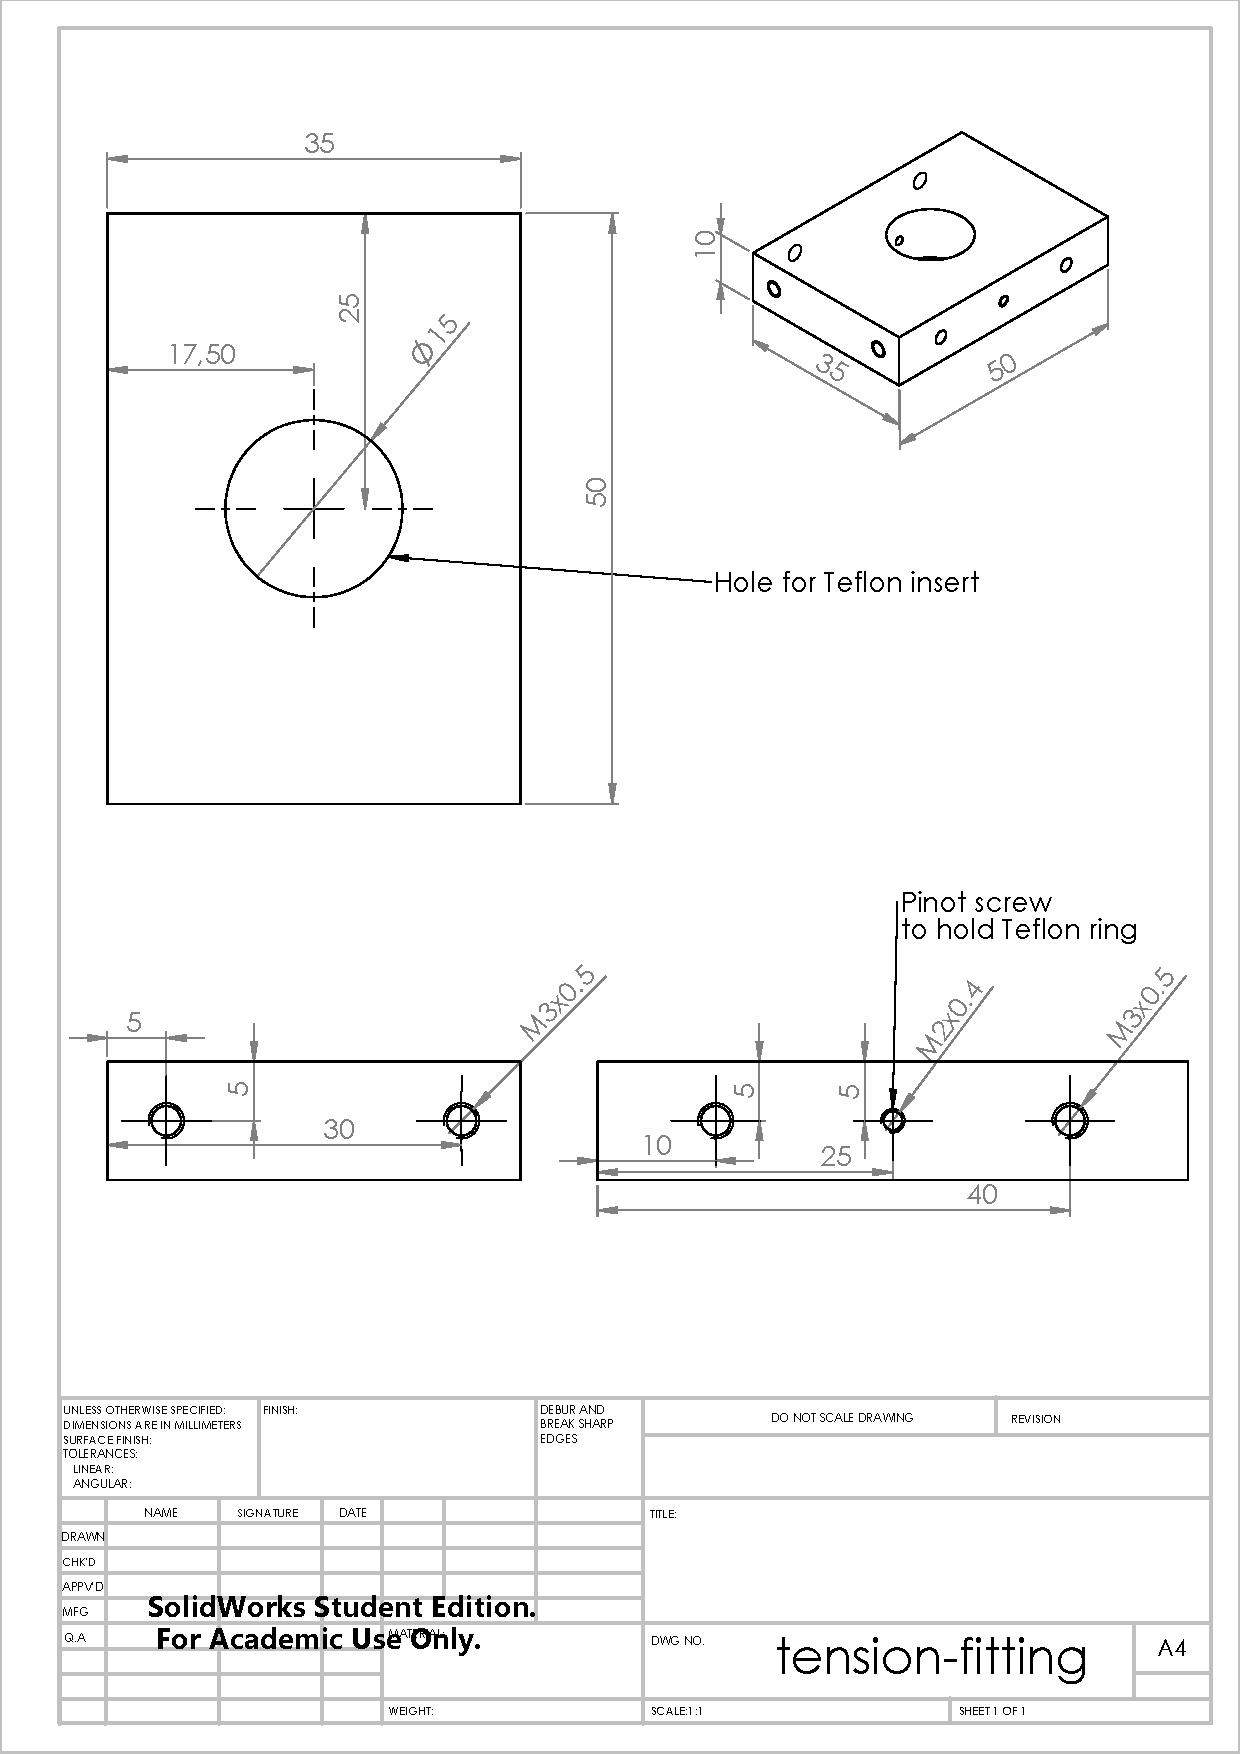
\includepdf[pages={-}]{graphics/cad/tension-fitting.pdf}
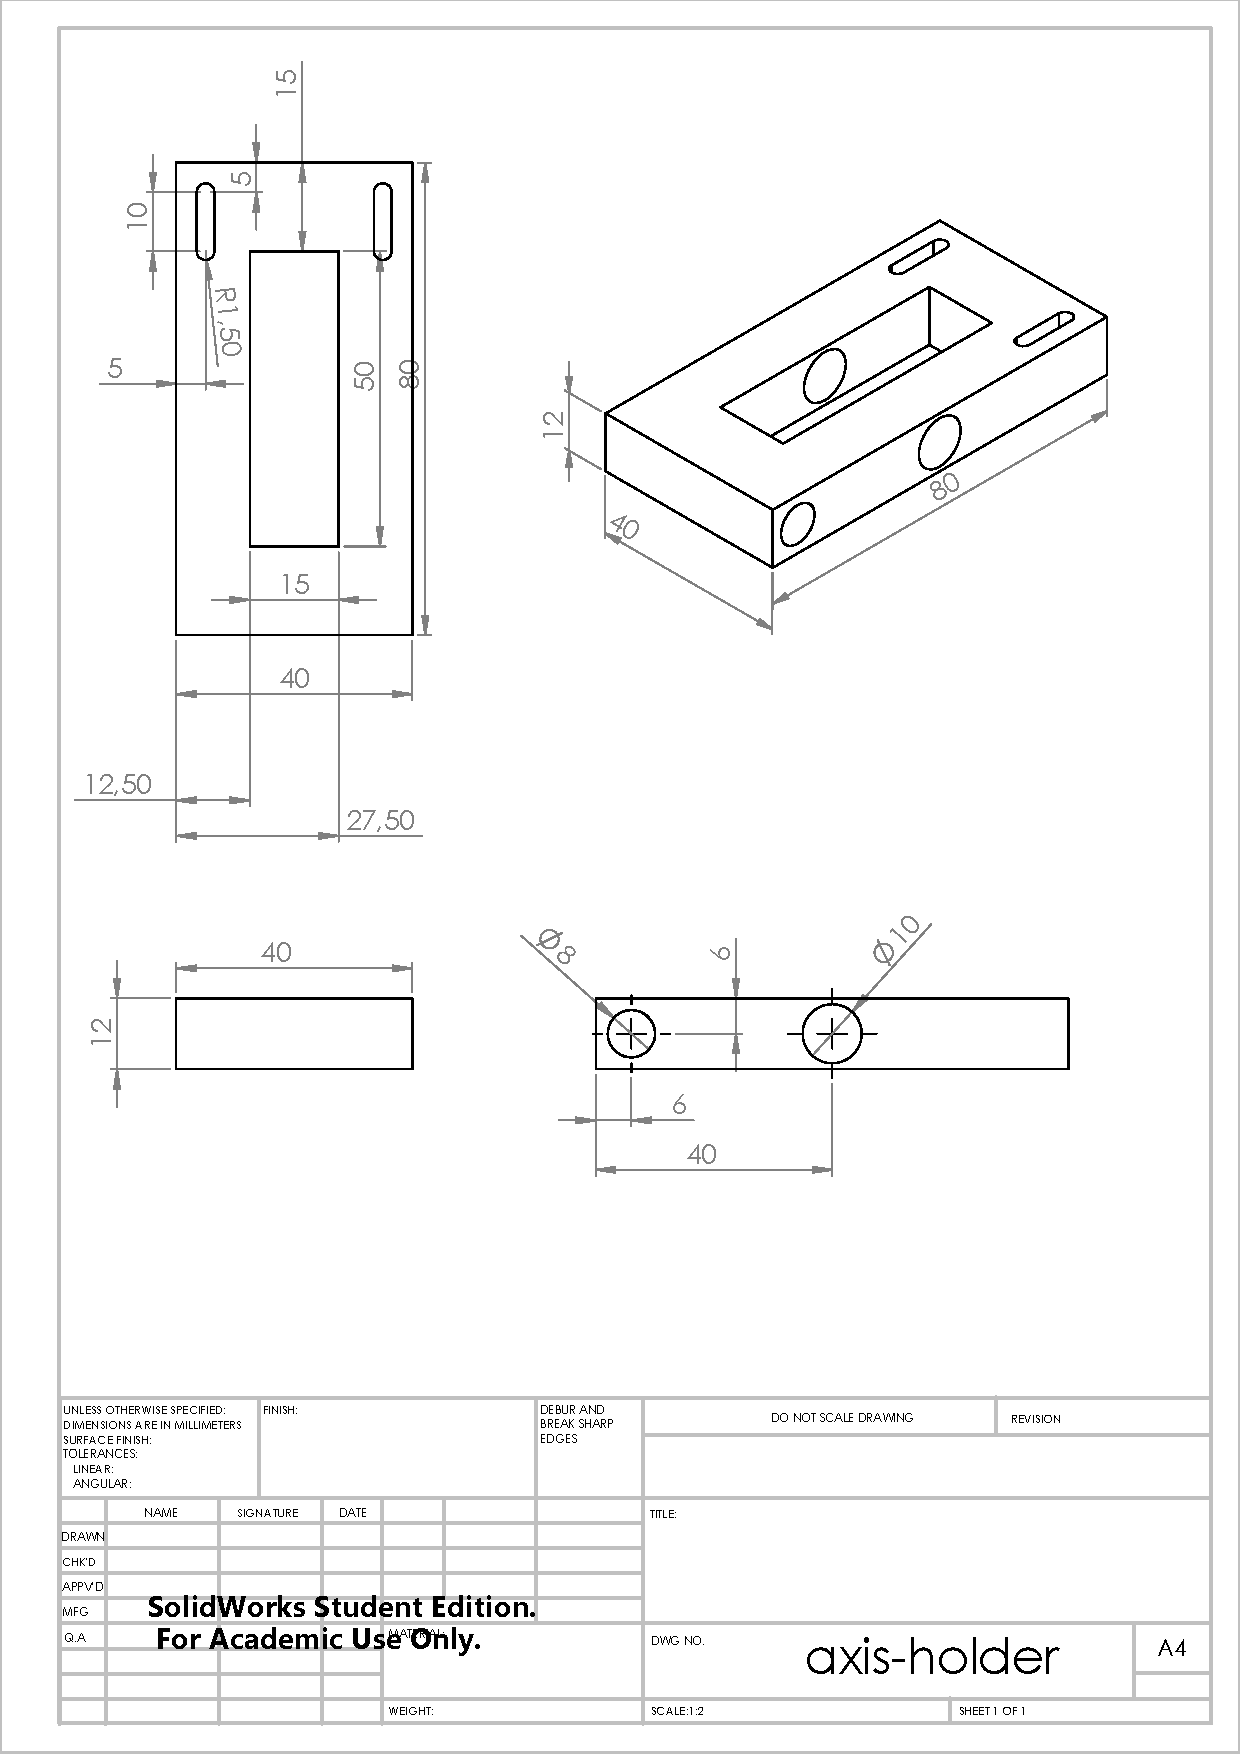
\includepdf[pages={-}]{graphics/cad/axis-holder.pdf}
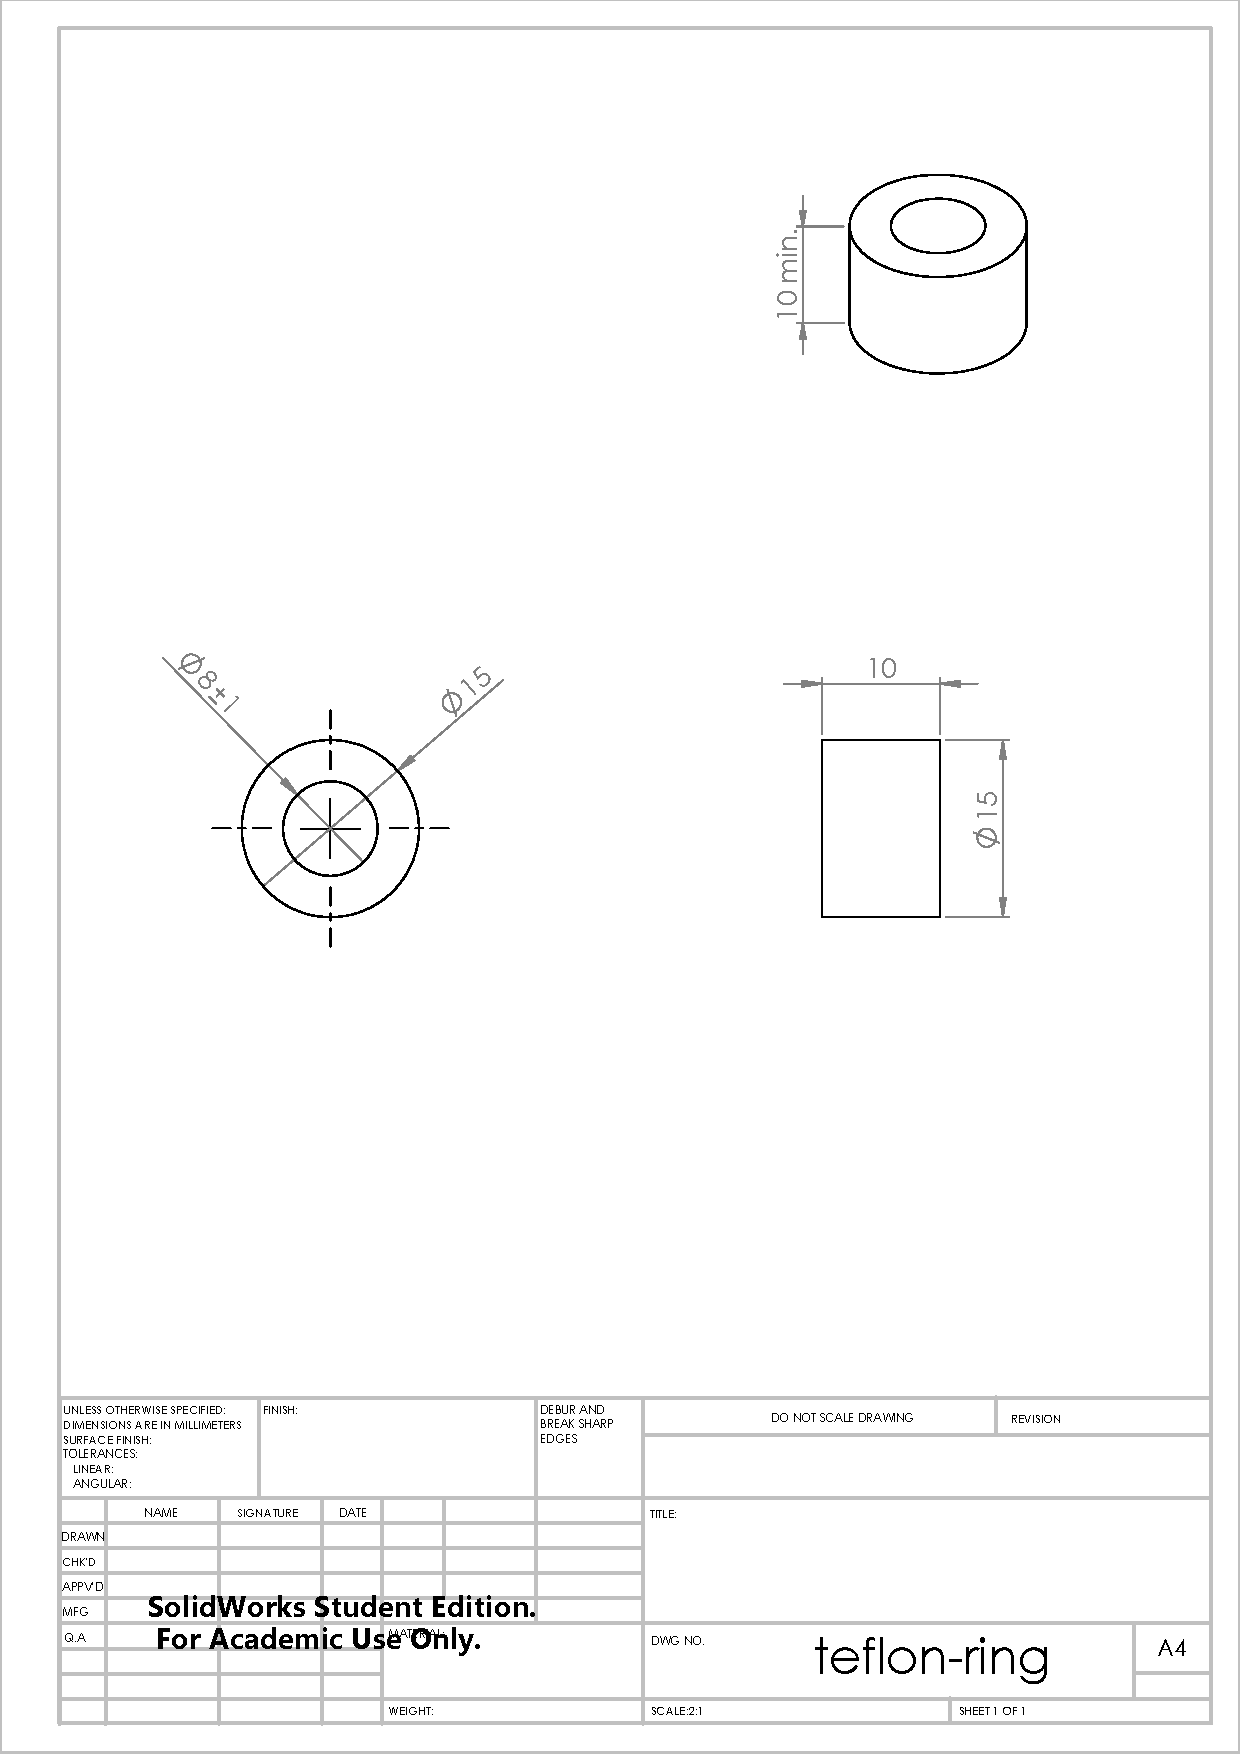
\includepdf[pages={-}]{graphics/cad/teflon-ring.pdf}
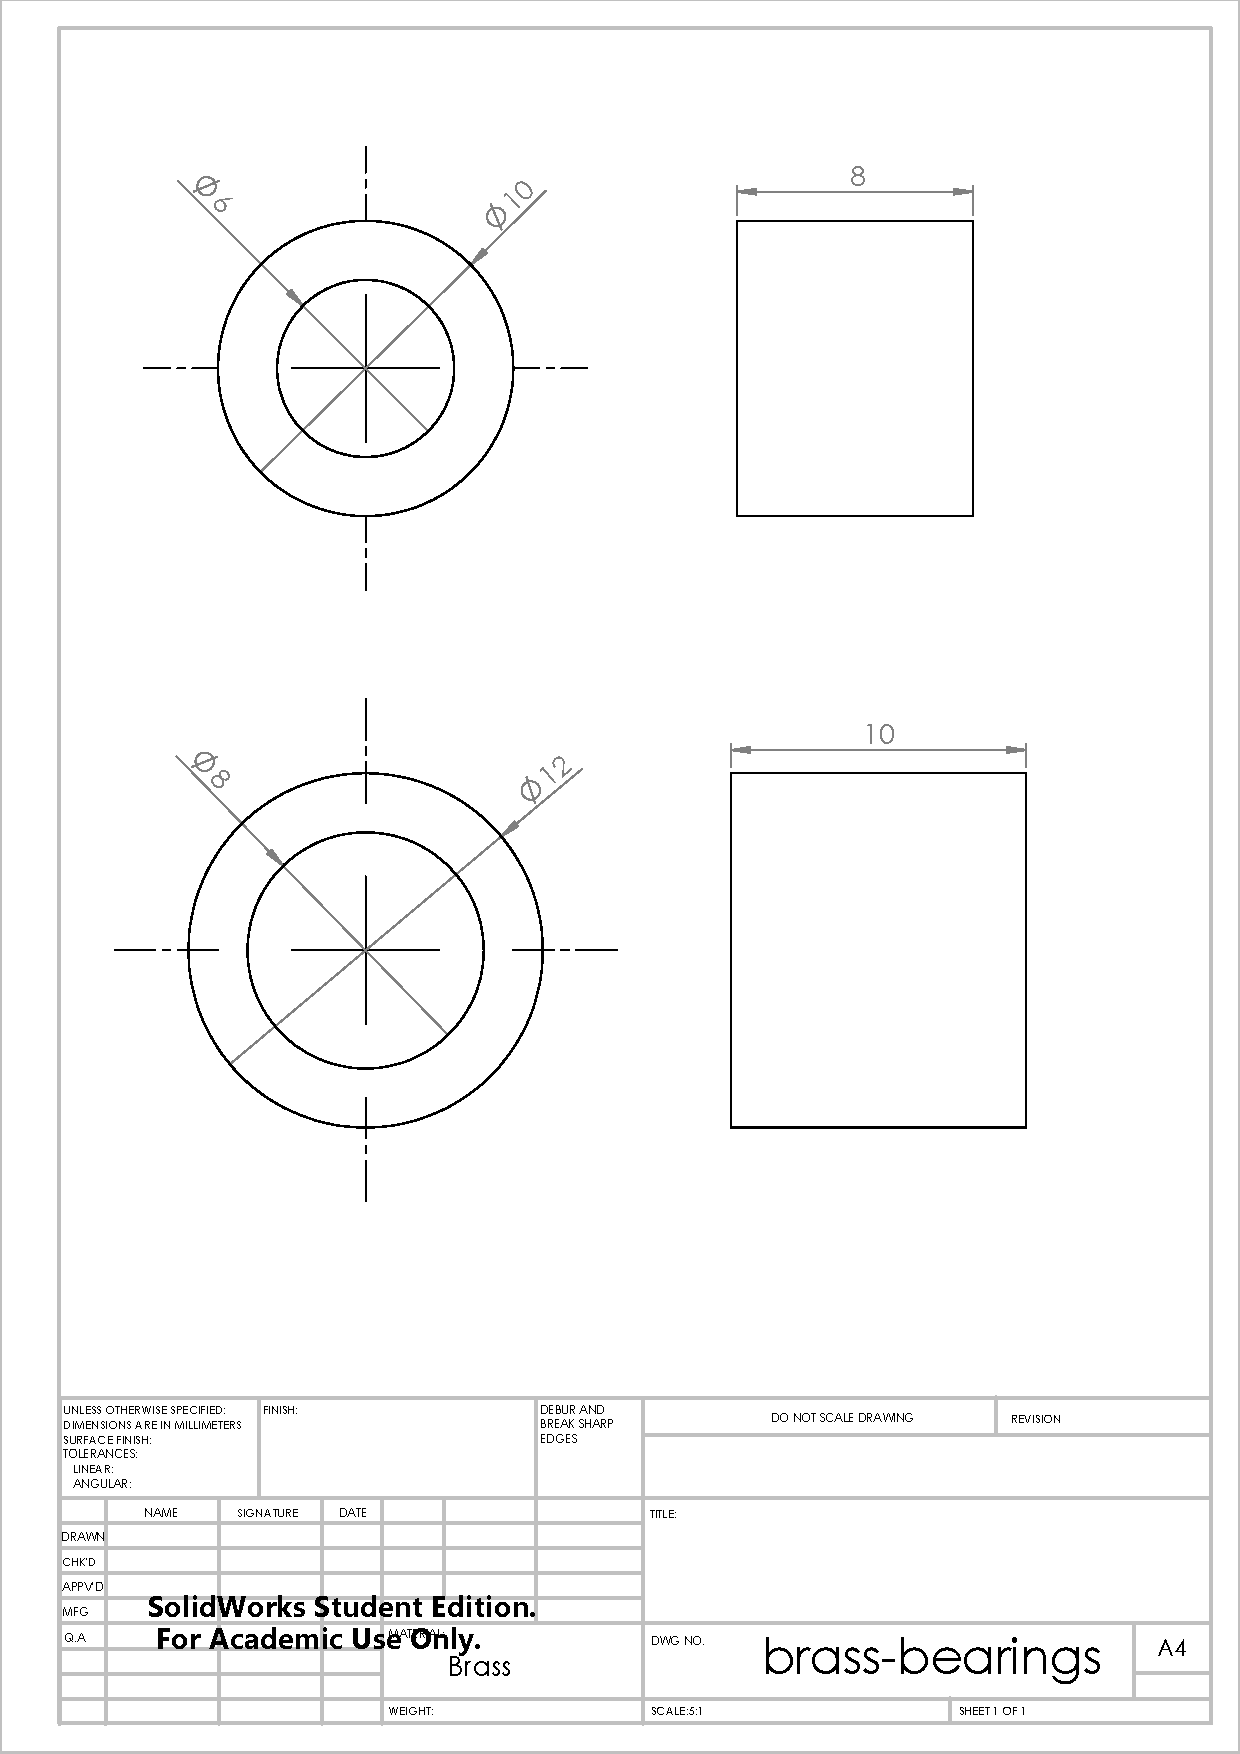
\includepdf[pages={-}]{graphics/cad/brass-bearings.pdf}
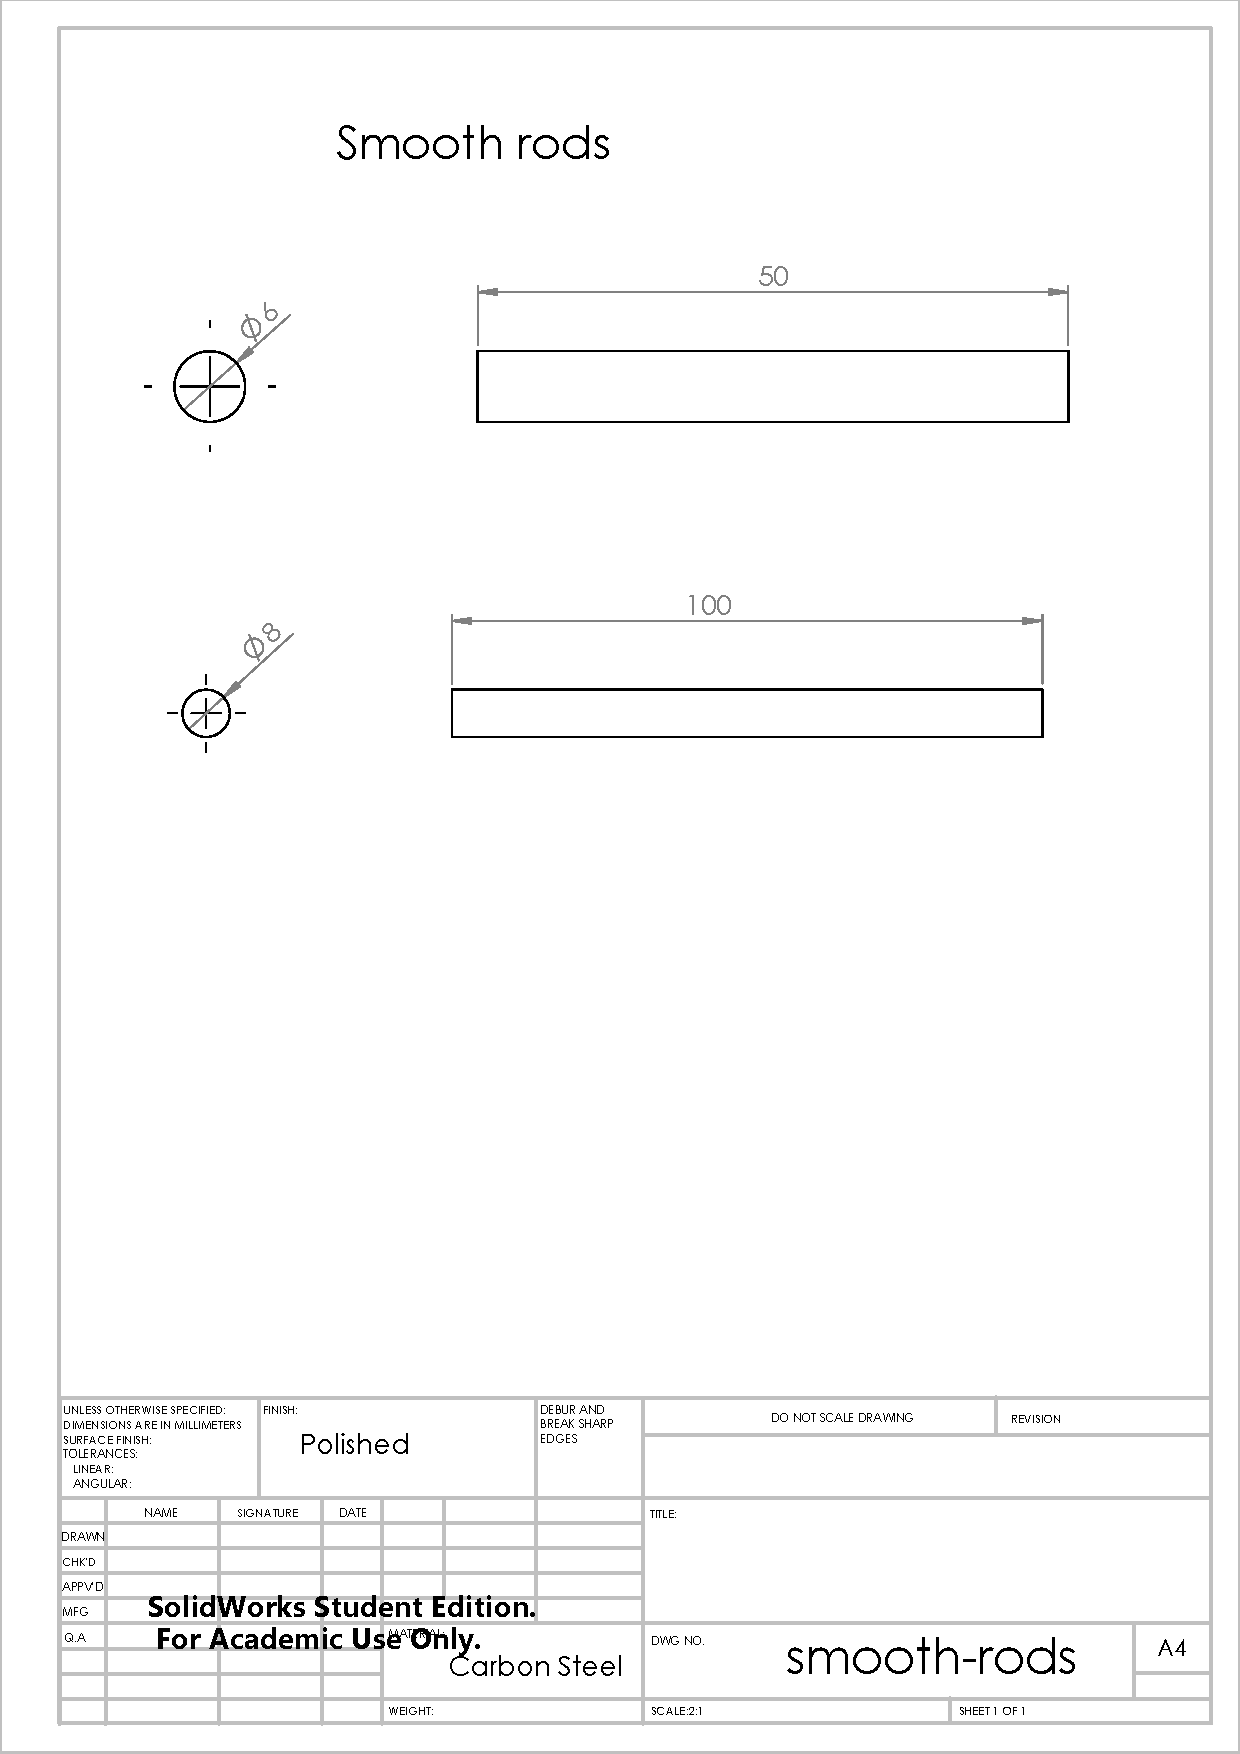
\includepdf[pages={-}]{graphics/cad/smooth-rods.pdf}

\subsection{The Cable Drum}

The Cable Drum is the most developed and complex prototype of the two winching methods. It has 3 motors, 2 to turn the drum around and 1 to move the carrier from side to side. Again it is very much inspired of open source 3d printers\footnote{Reprep open source 3d printers, www.reprap.org.}. Every thing can be mounted to the bottom of the helipad. \\
The power is connected to the drum through 2 slips rings. The slip rings can't carry any payload since they are made of thin plastic. \\
The drum has 4 big holes in the vertical direction to help passive heat dissipation from the cable.

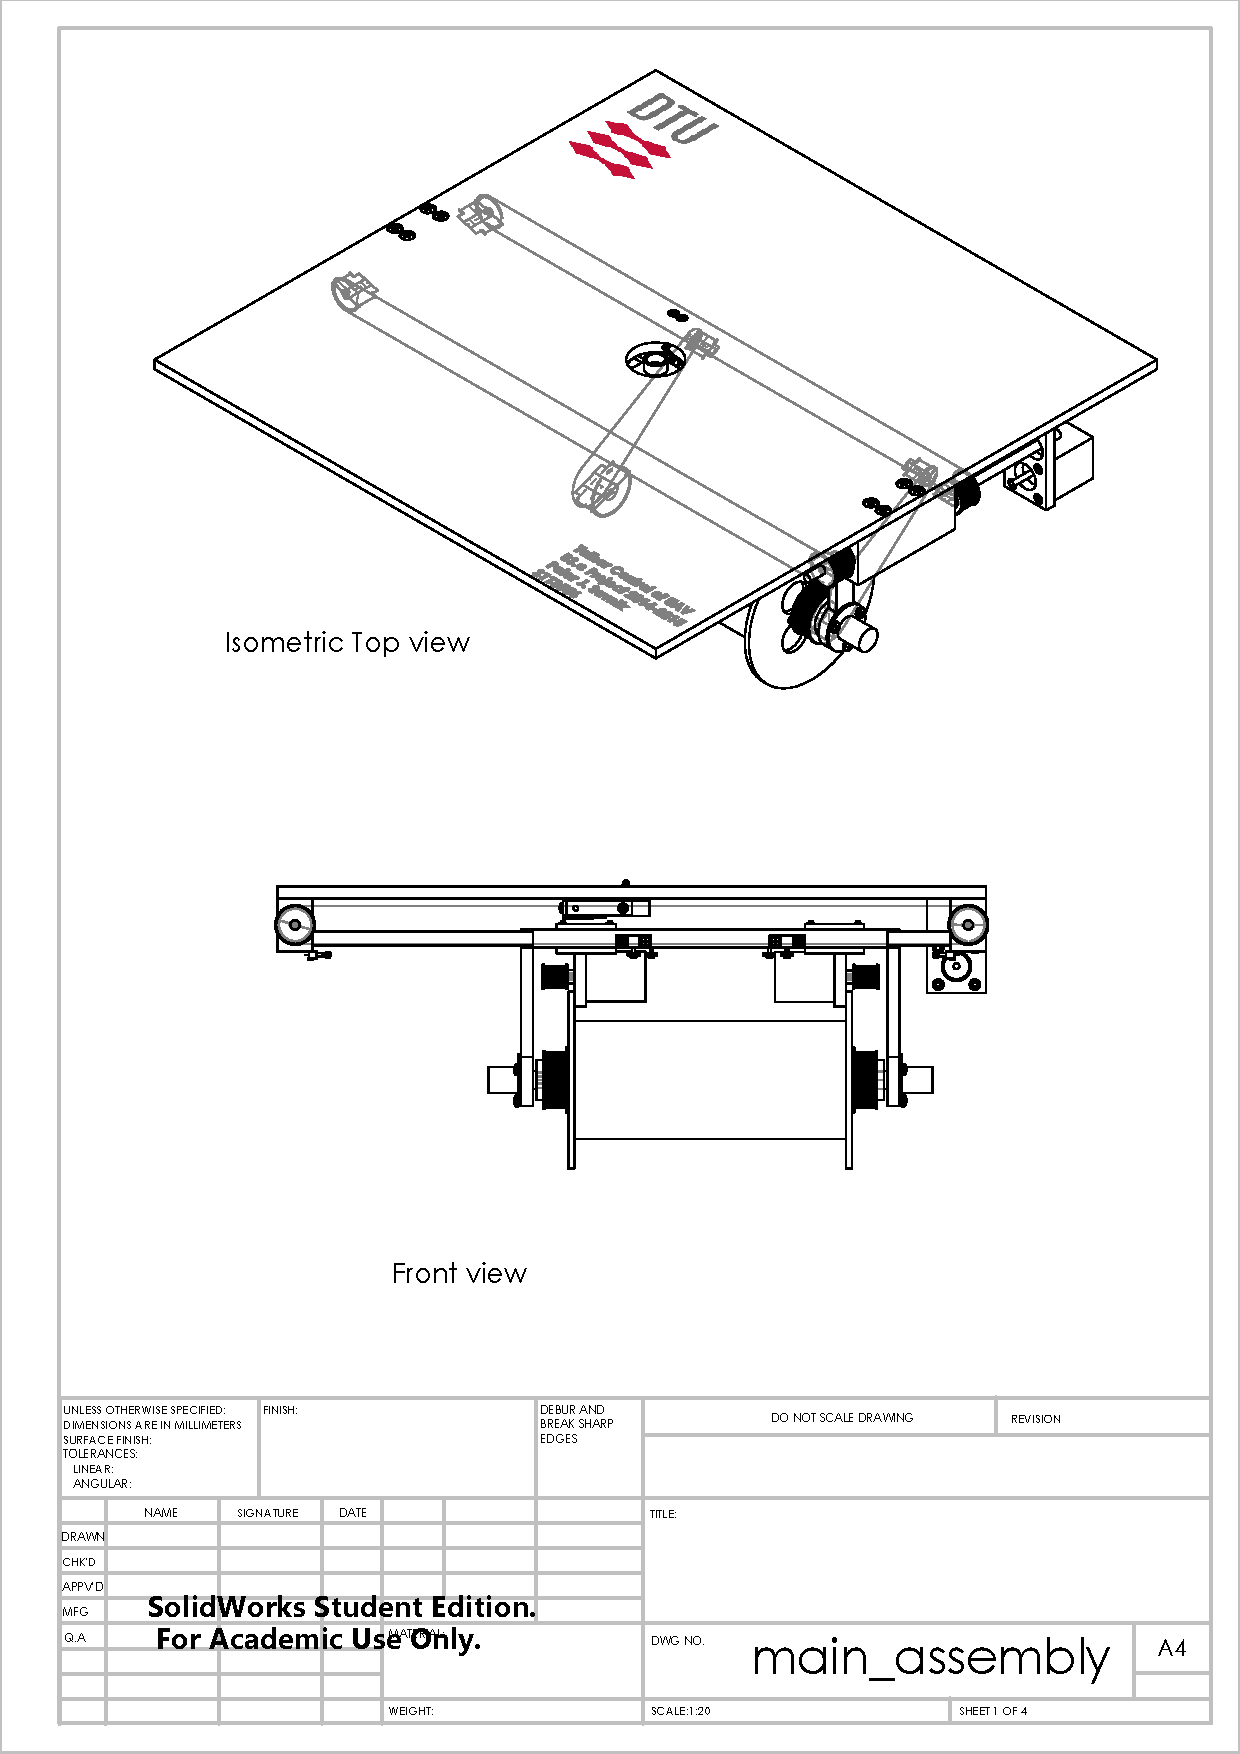
\includepdf[pages={-}]{graphics/cad/main_assembly_3.pdf}
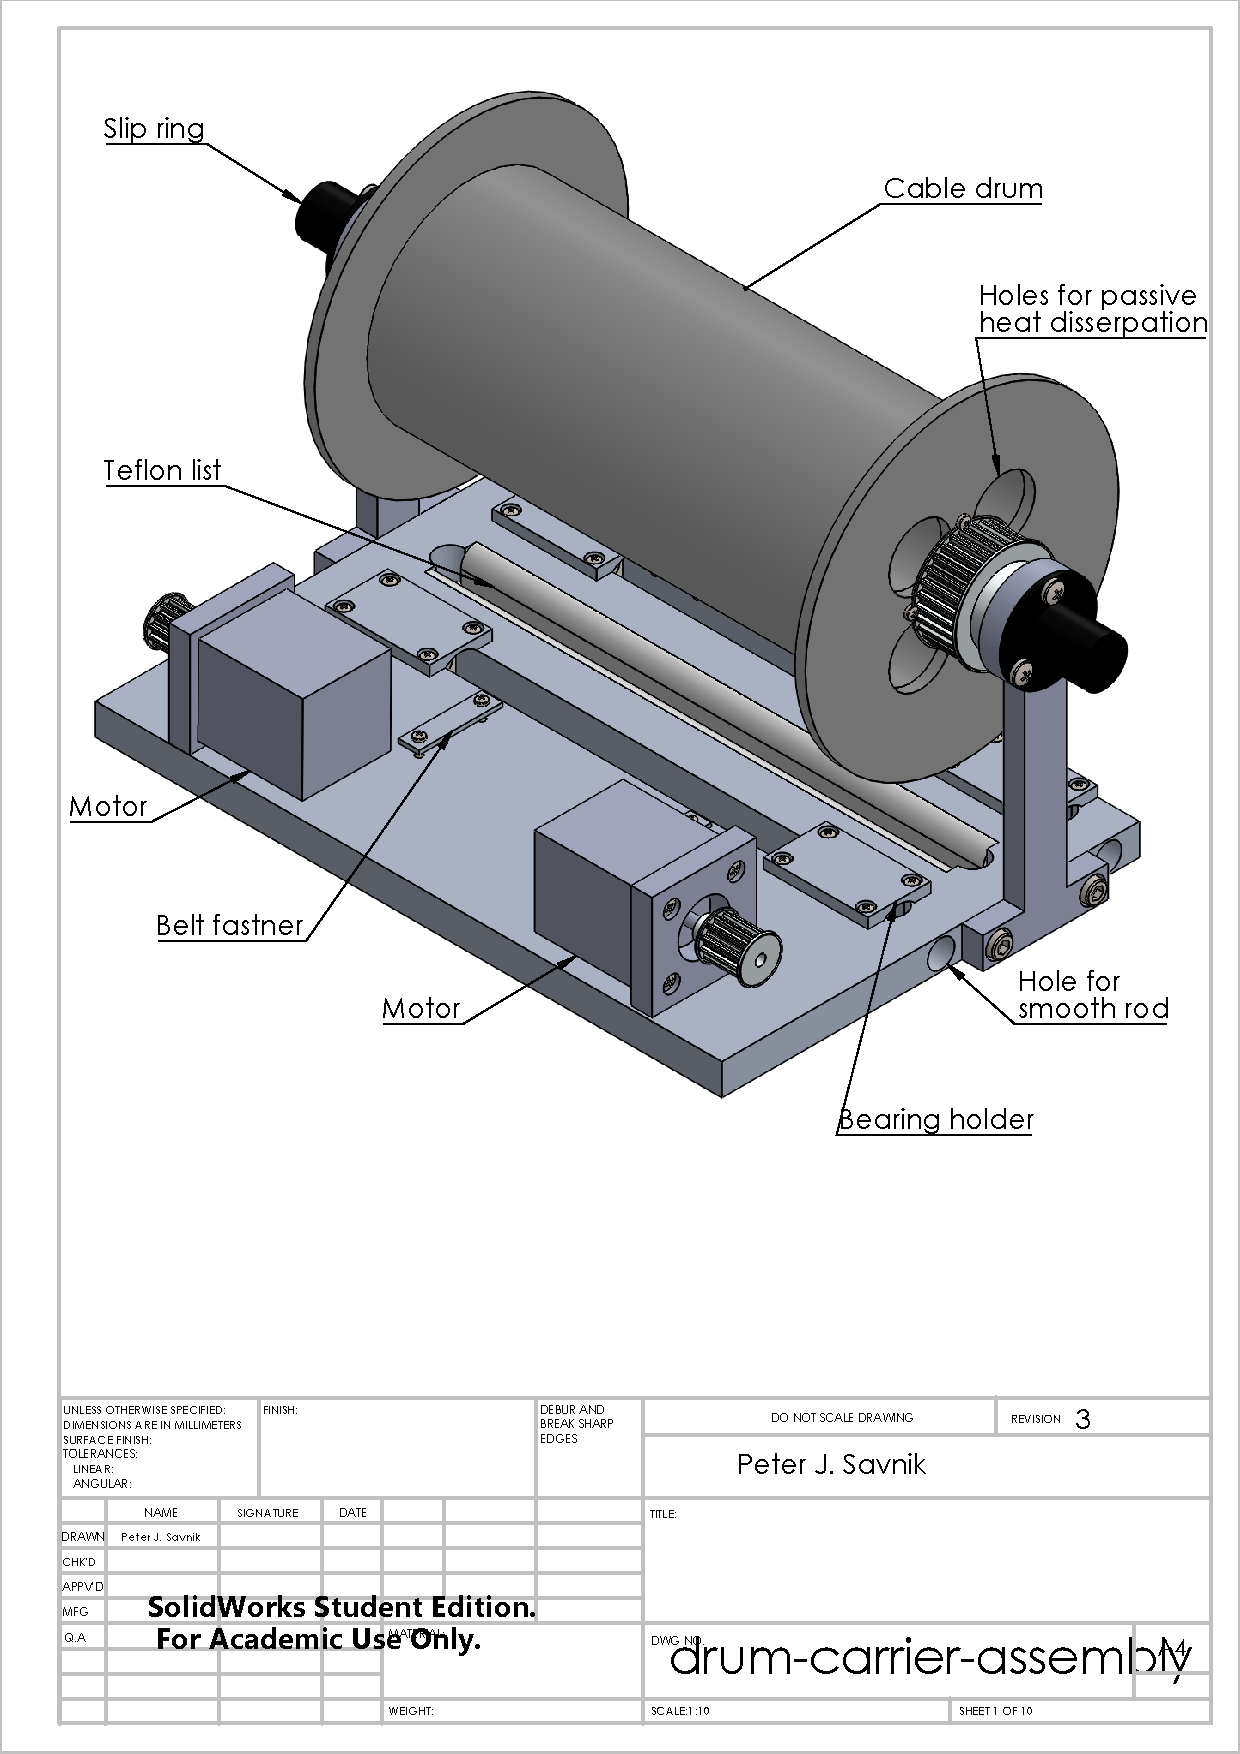
\includepdf[pages={-}]{graphics/cad/drum-carrier-assembly.pdf}
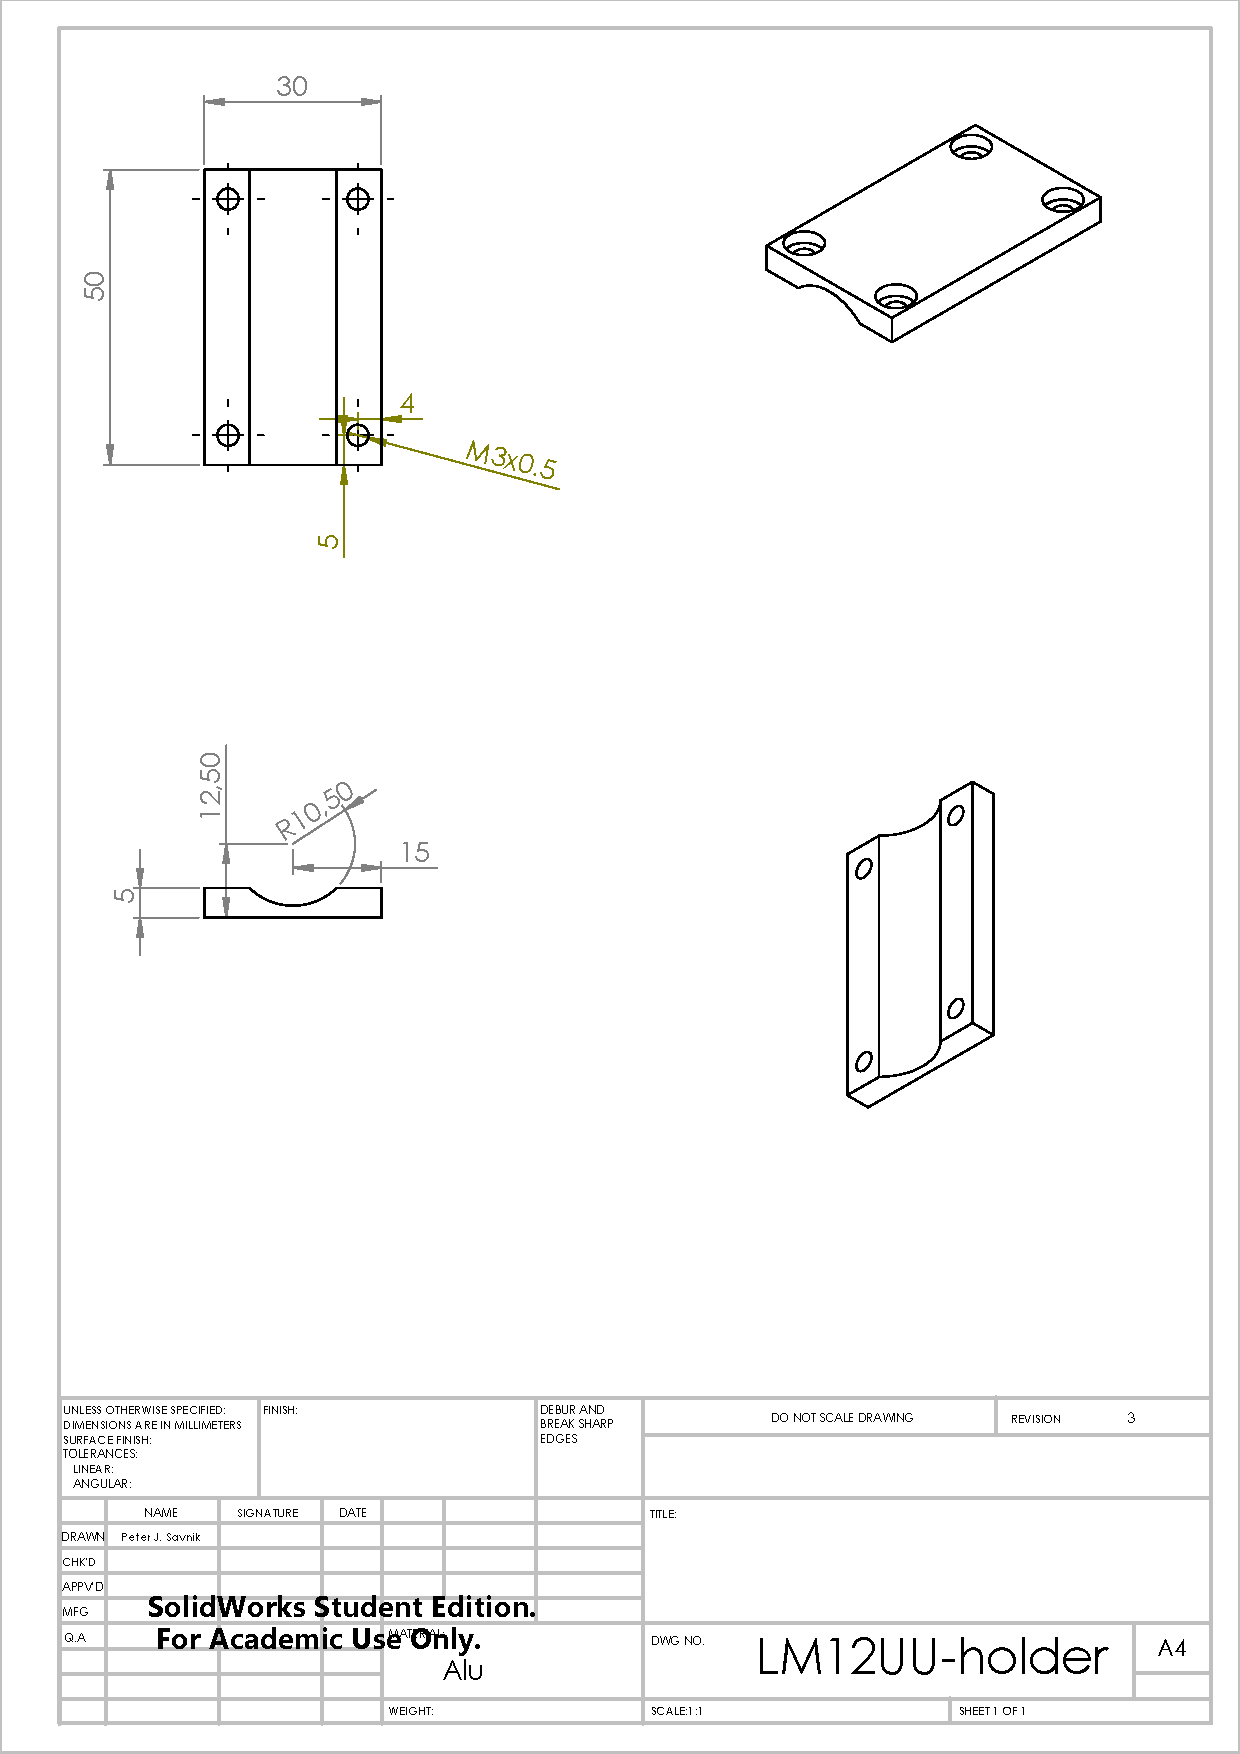
\includepdf[pages={-}]{graphics/cad/LM12UU-holder.pdf}
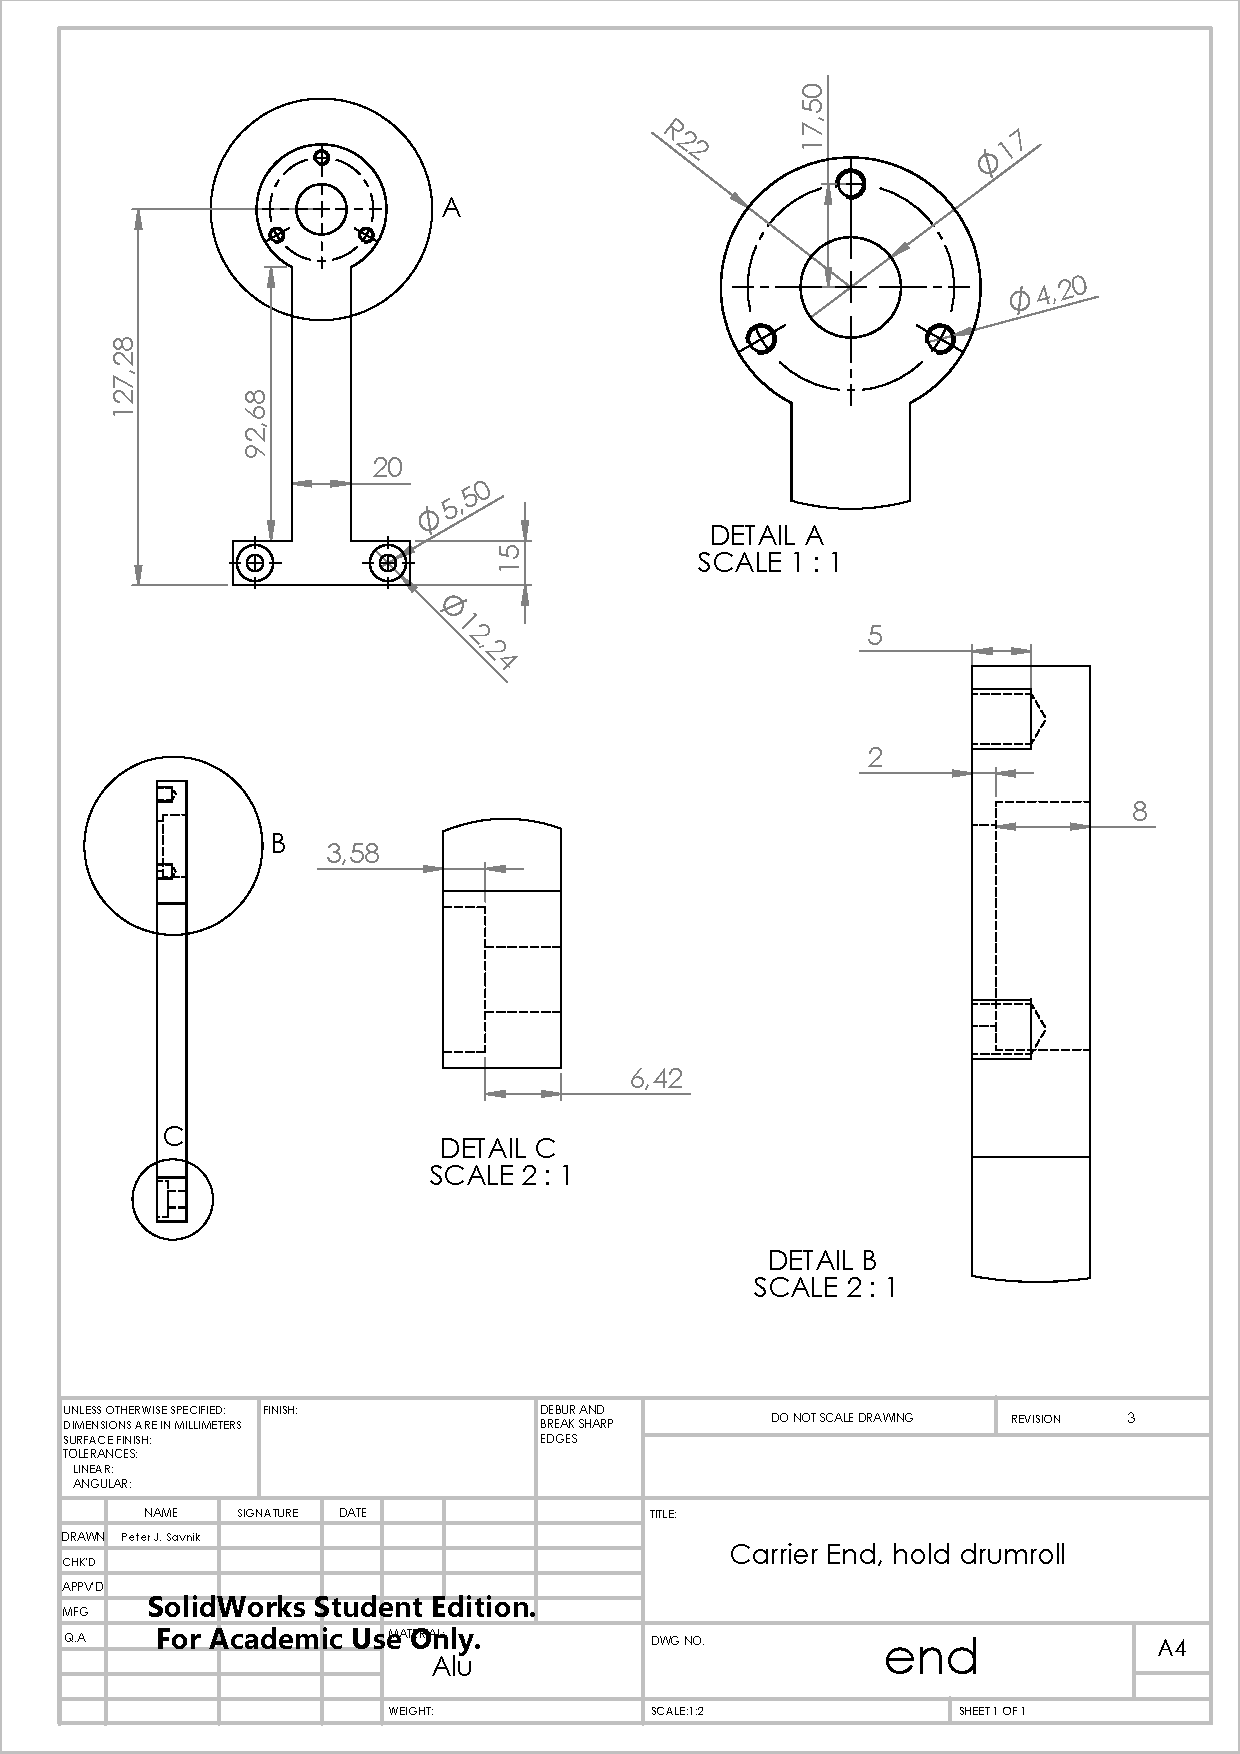
\includepdf[pages={-}]{graphics/cad/end.pdf}
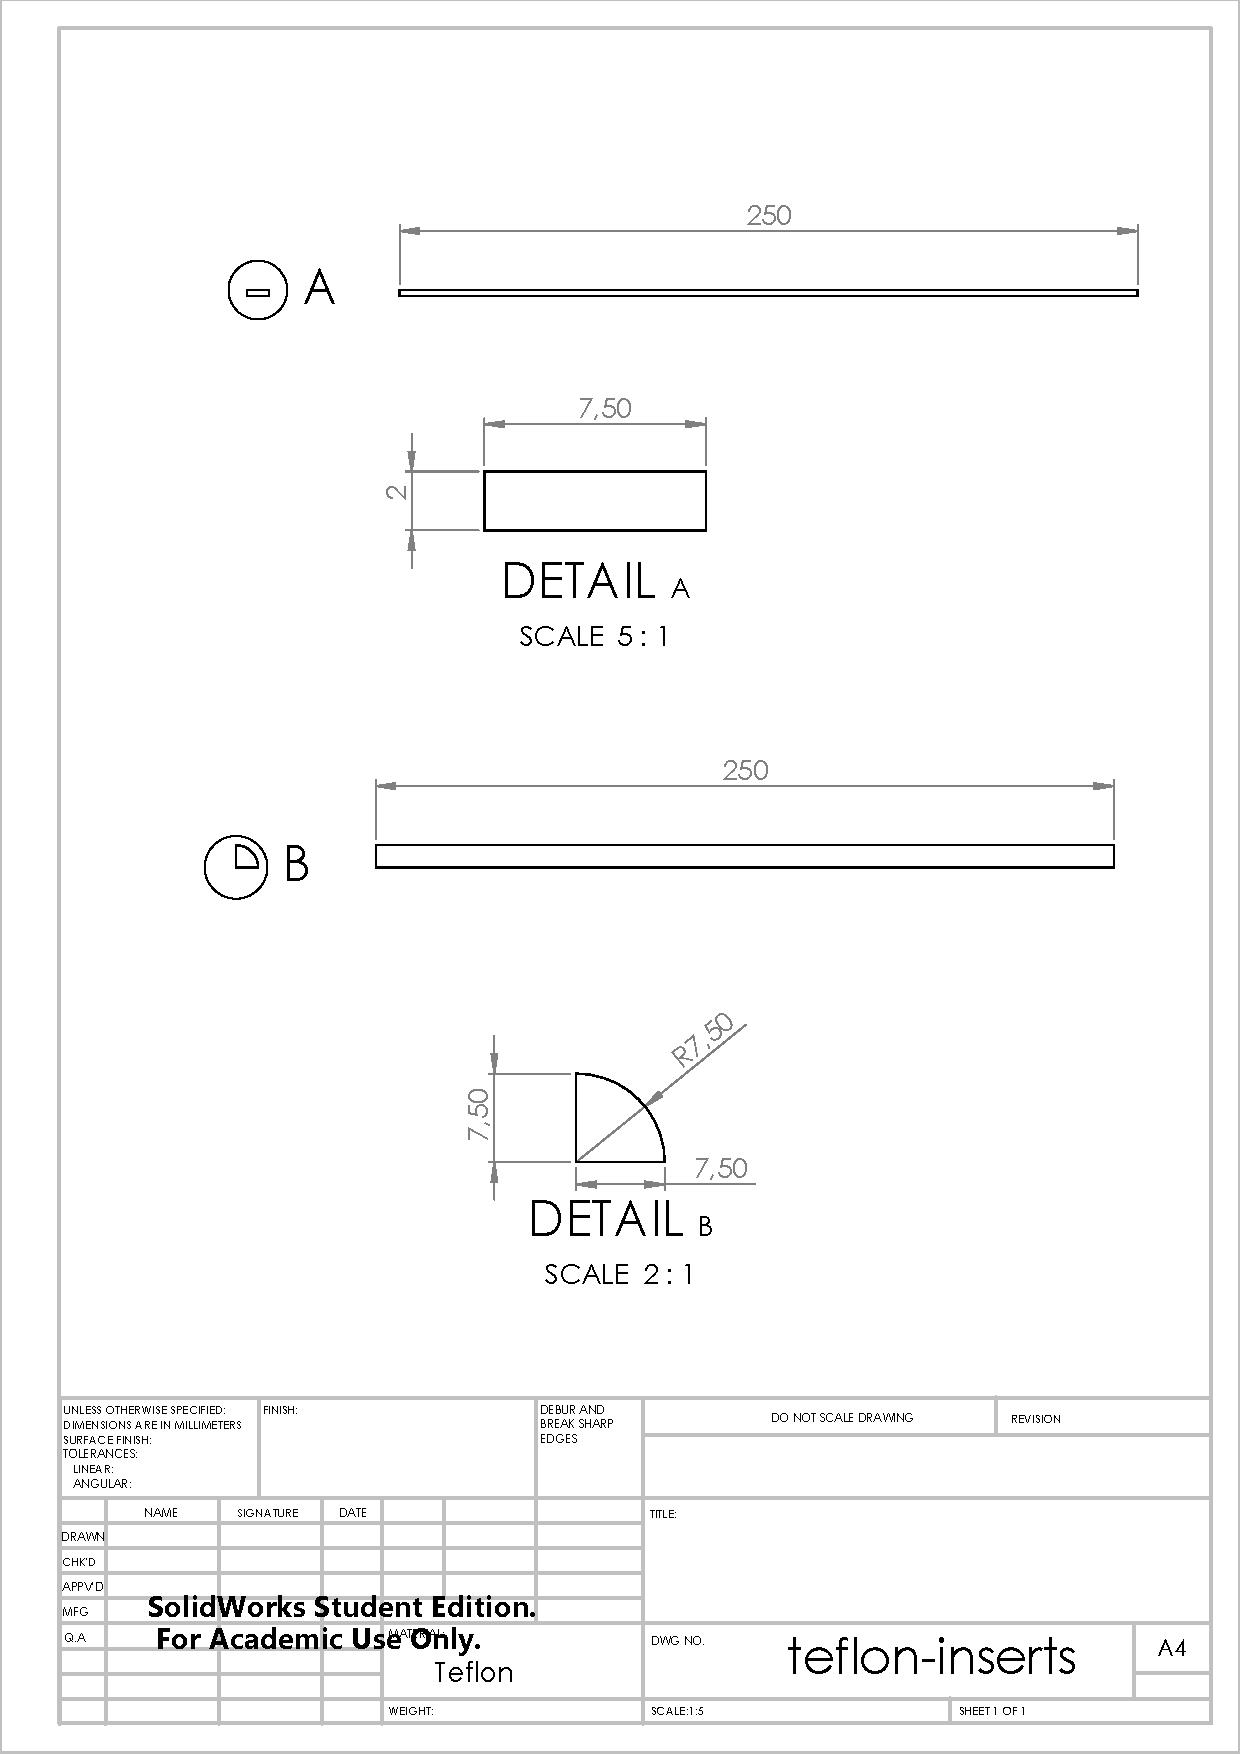
\includepdf[pages={-}]{graphics/cad/teflon-inserts.pdf}
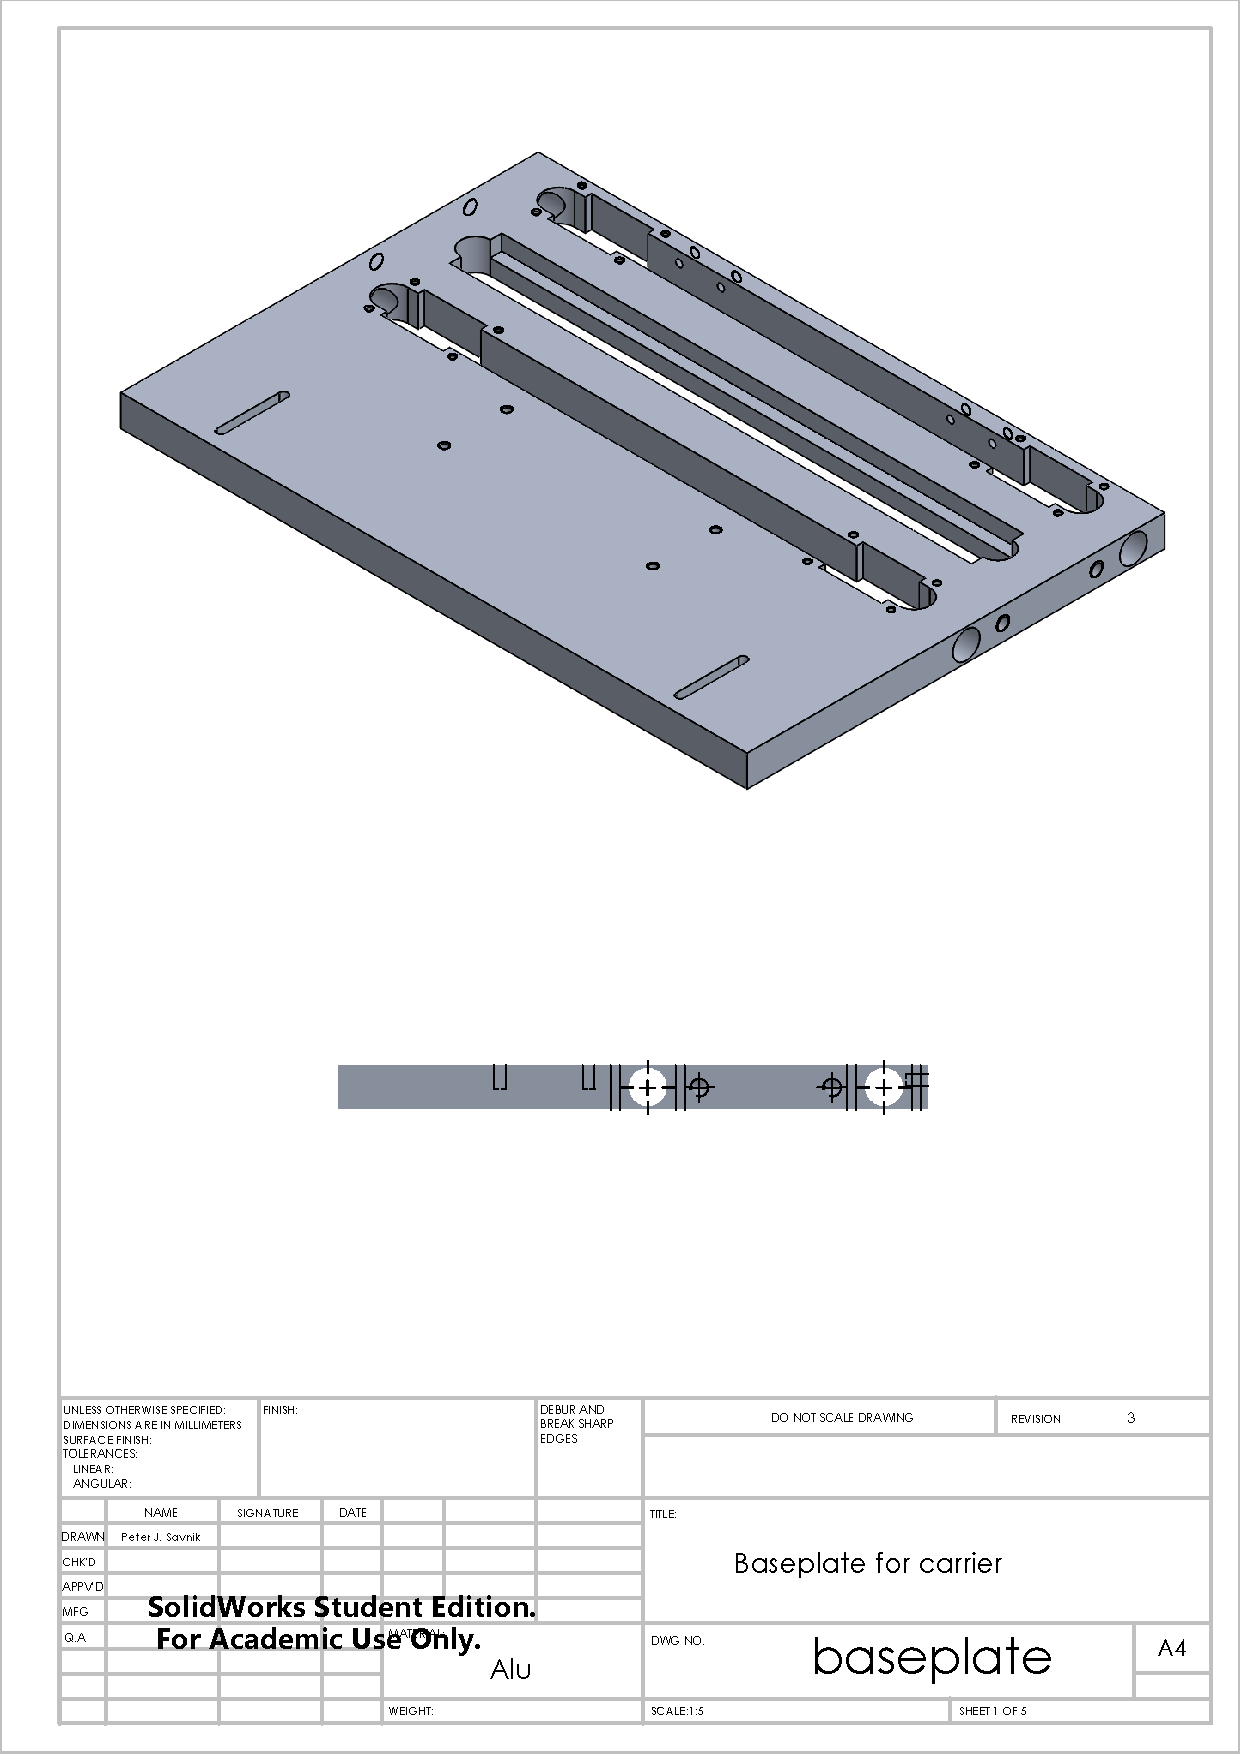
\includepdf[pages={-}]{graphics/cad/baseplate.pdf}
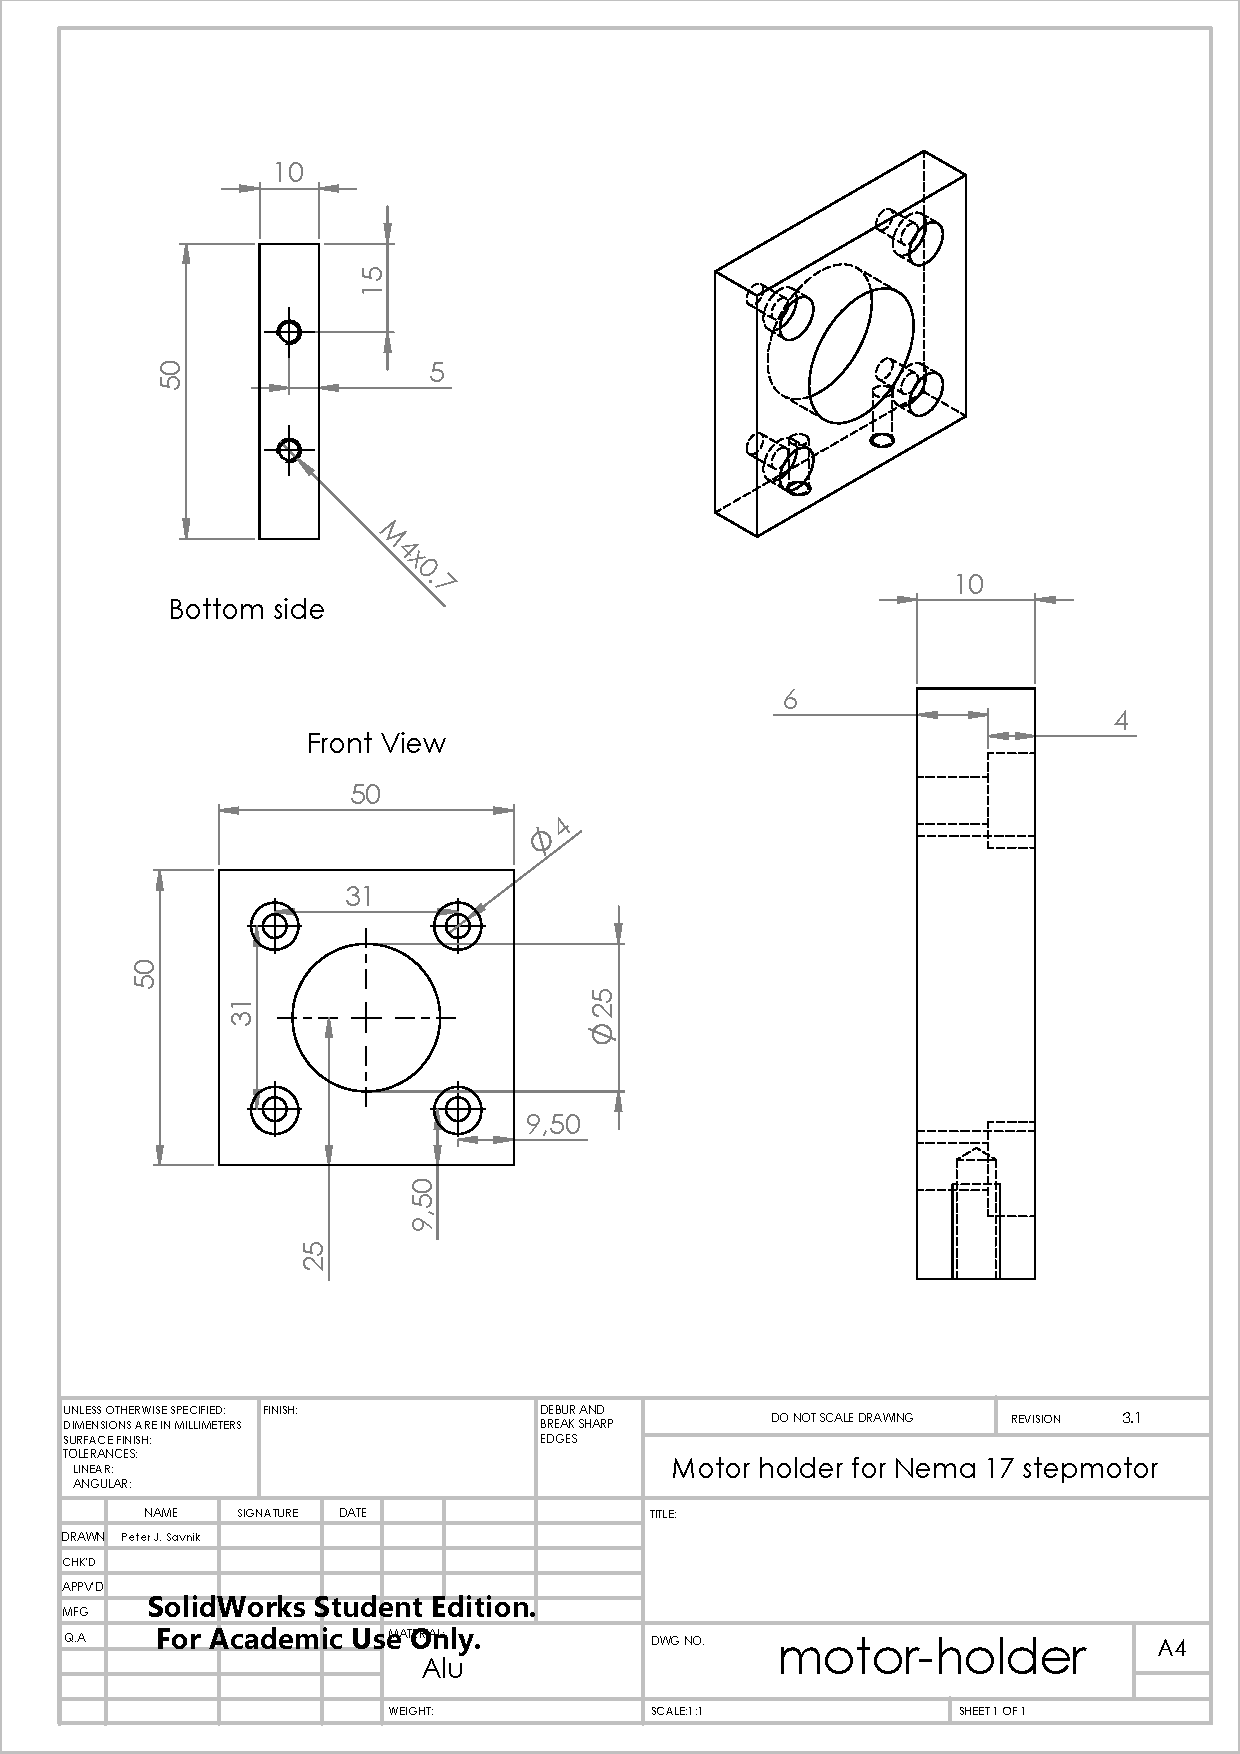
\includepdf[pages={-}]{graphics/cad/motor-holder.pdf}
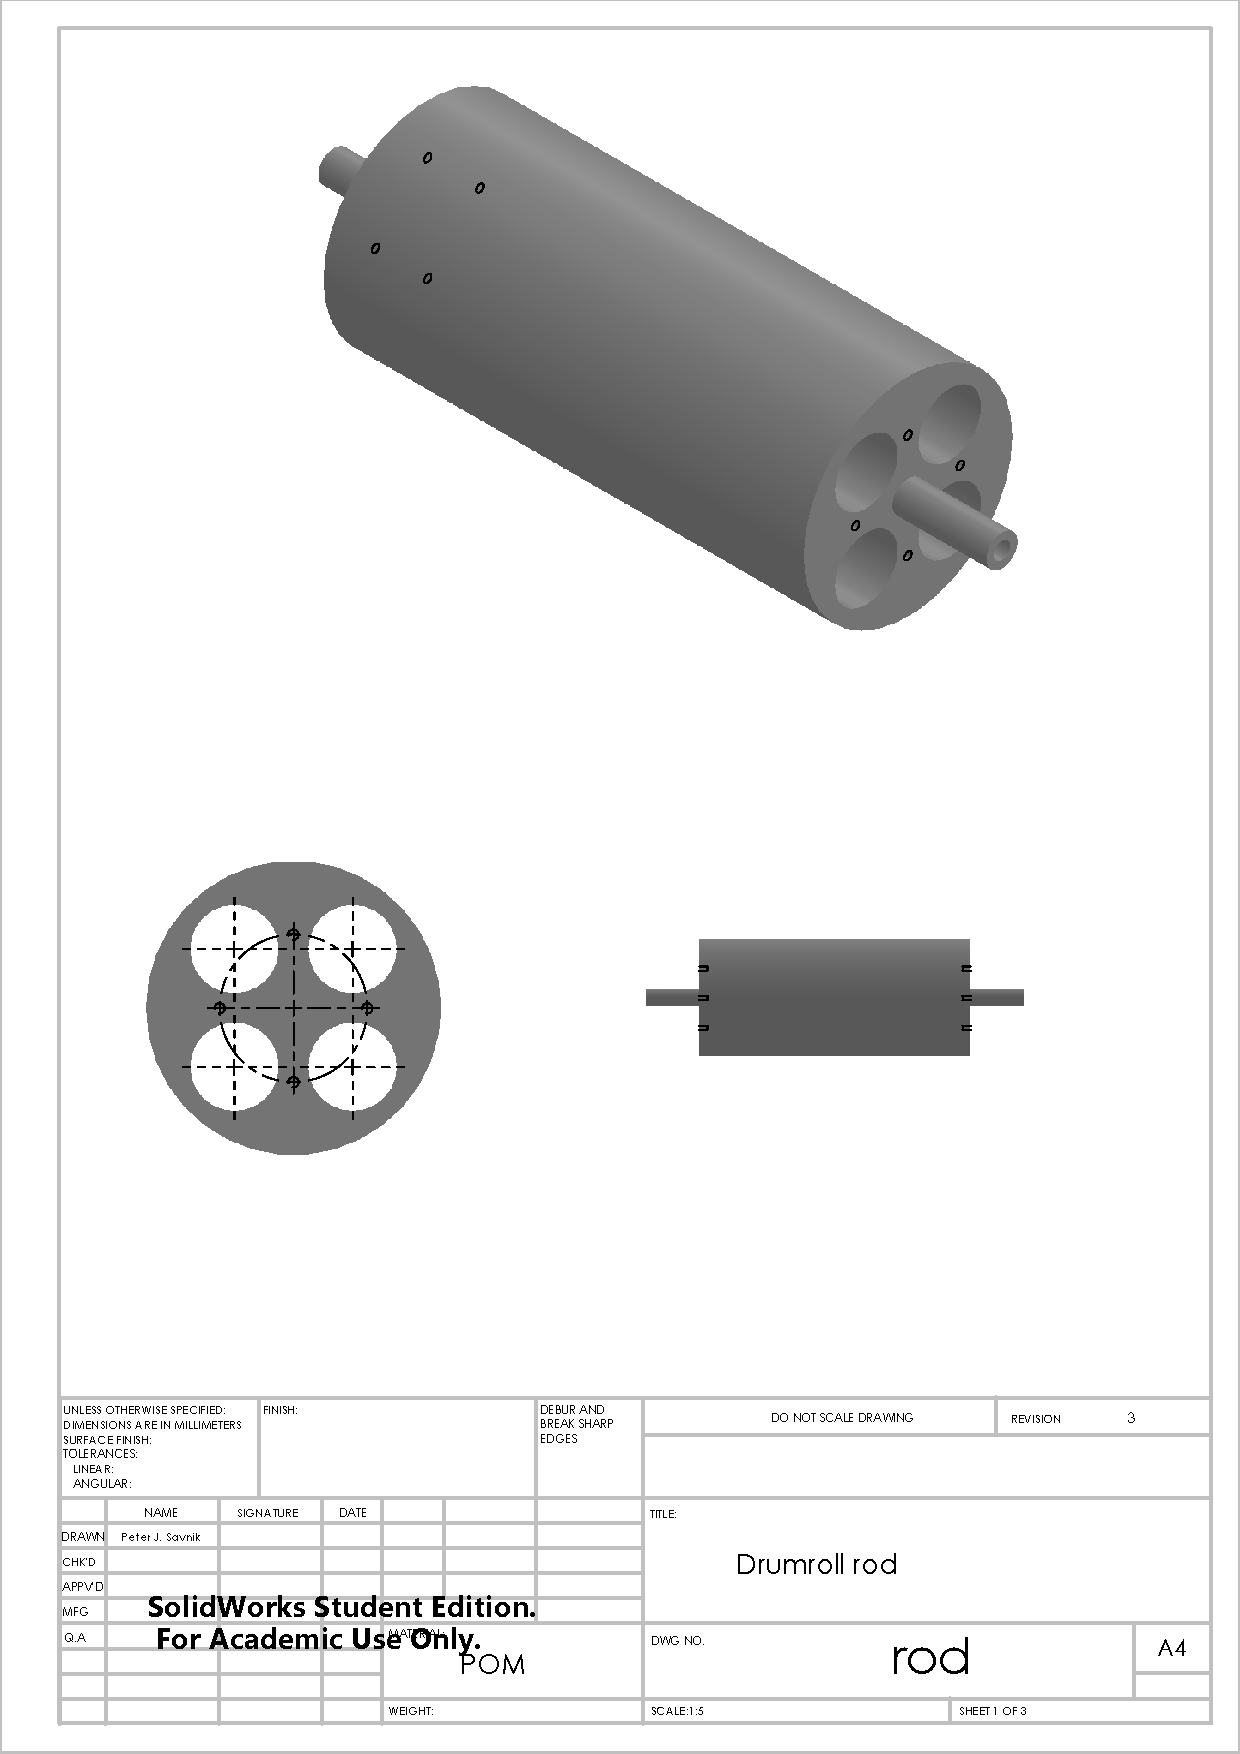
\includepdf[pages={-}]{graphics/cad/rod.pdf}
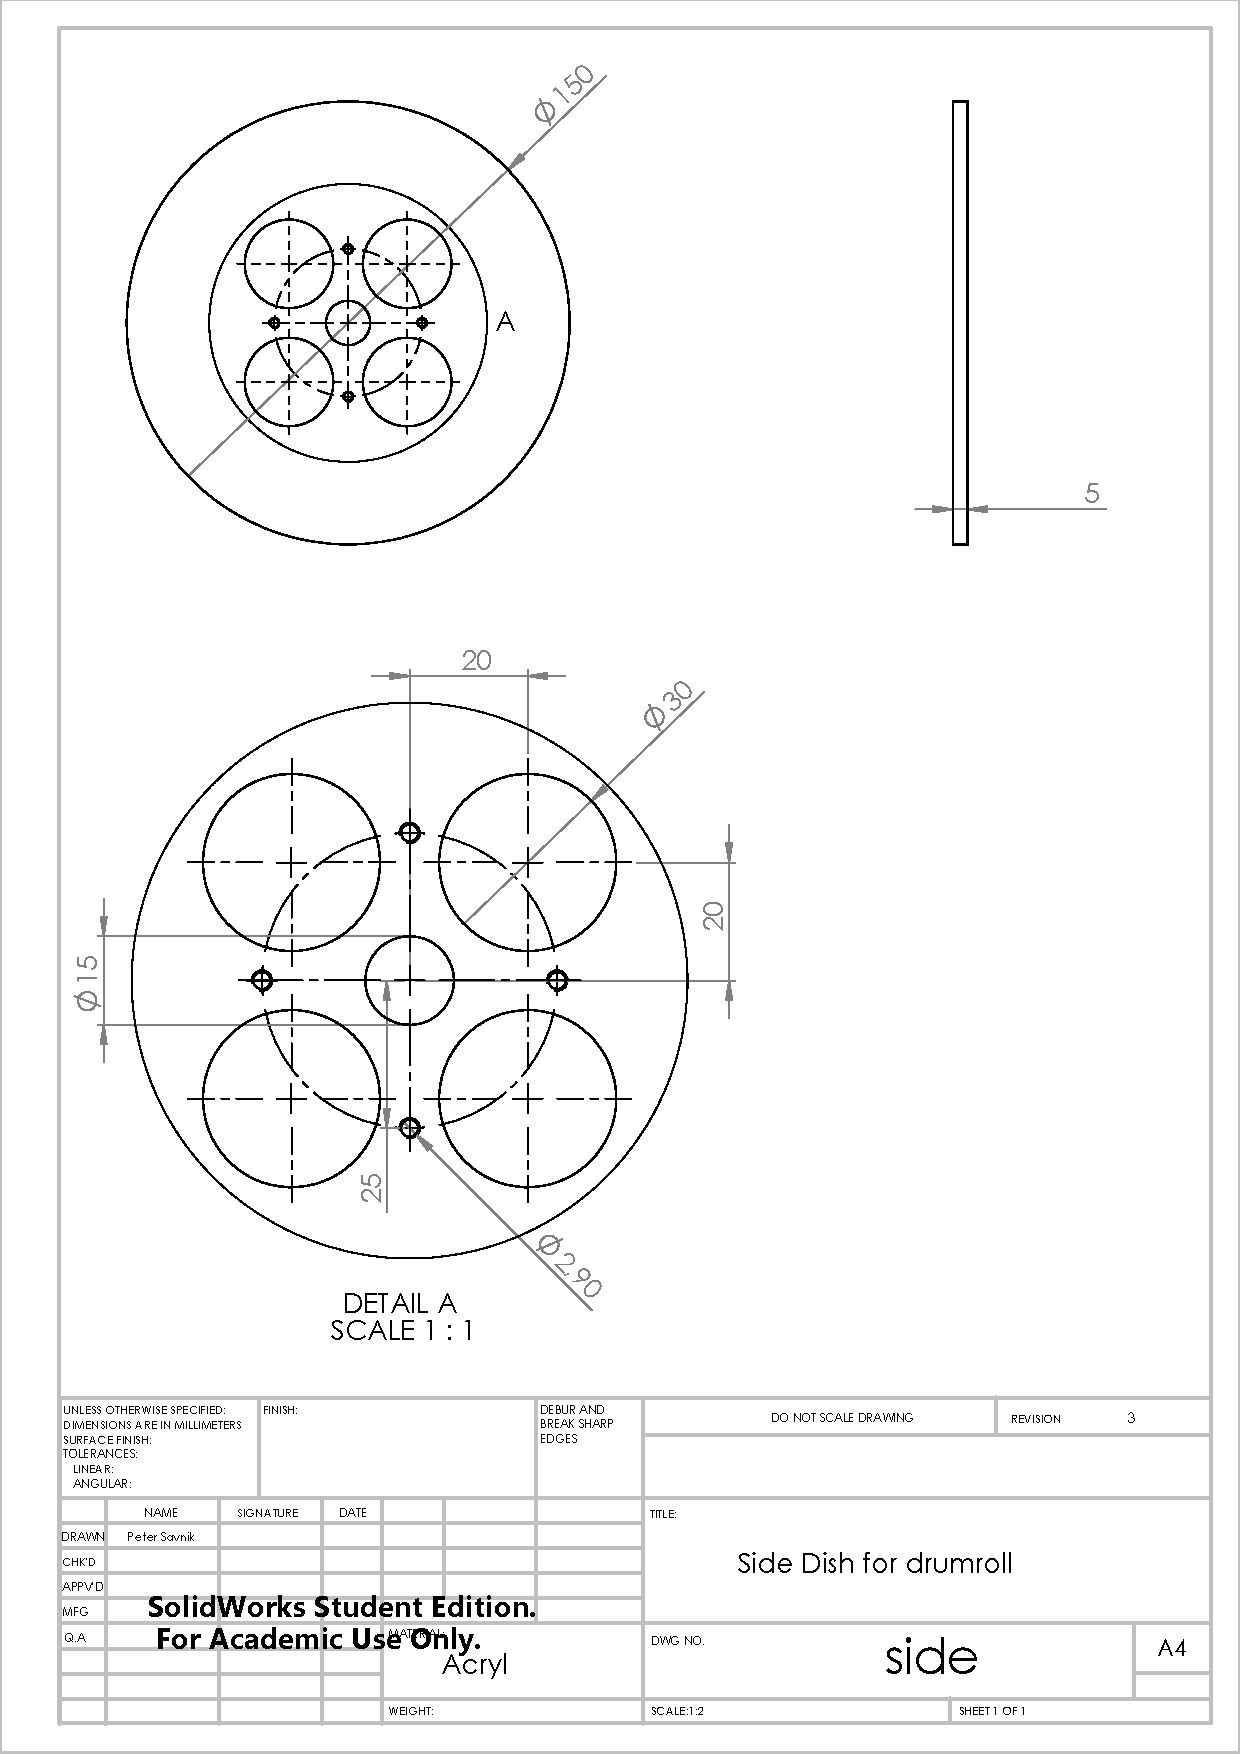
\includepdf[pages={-}]{graphics/cad/side.pdf}
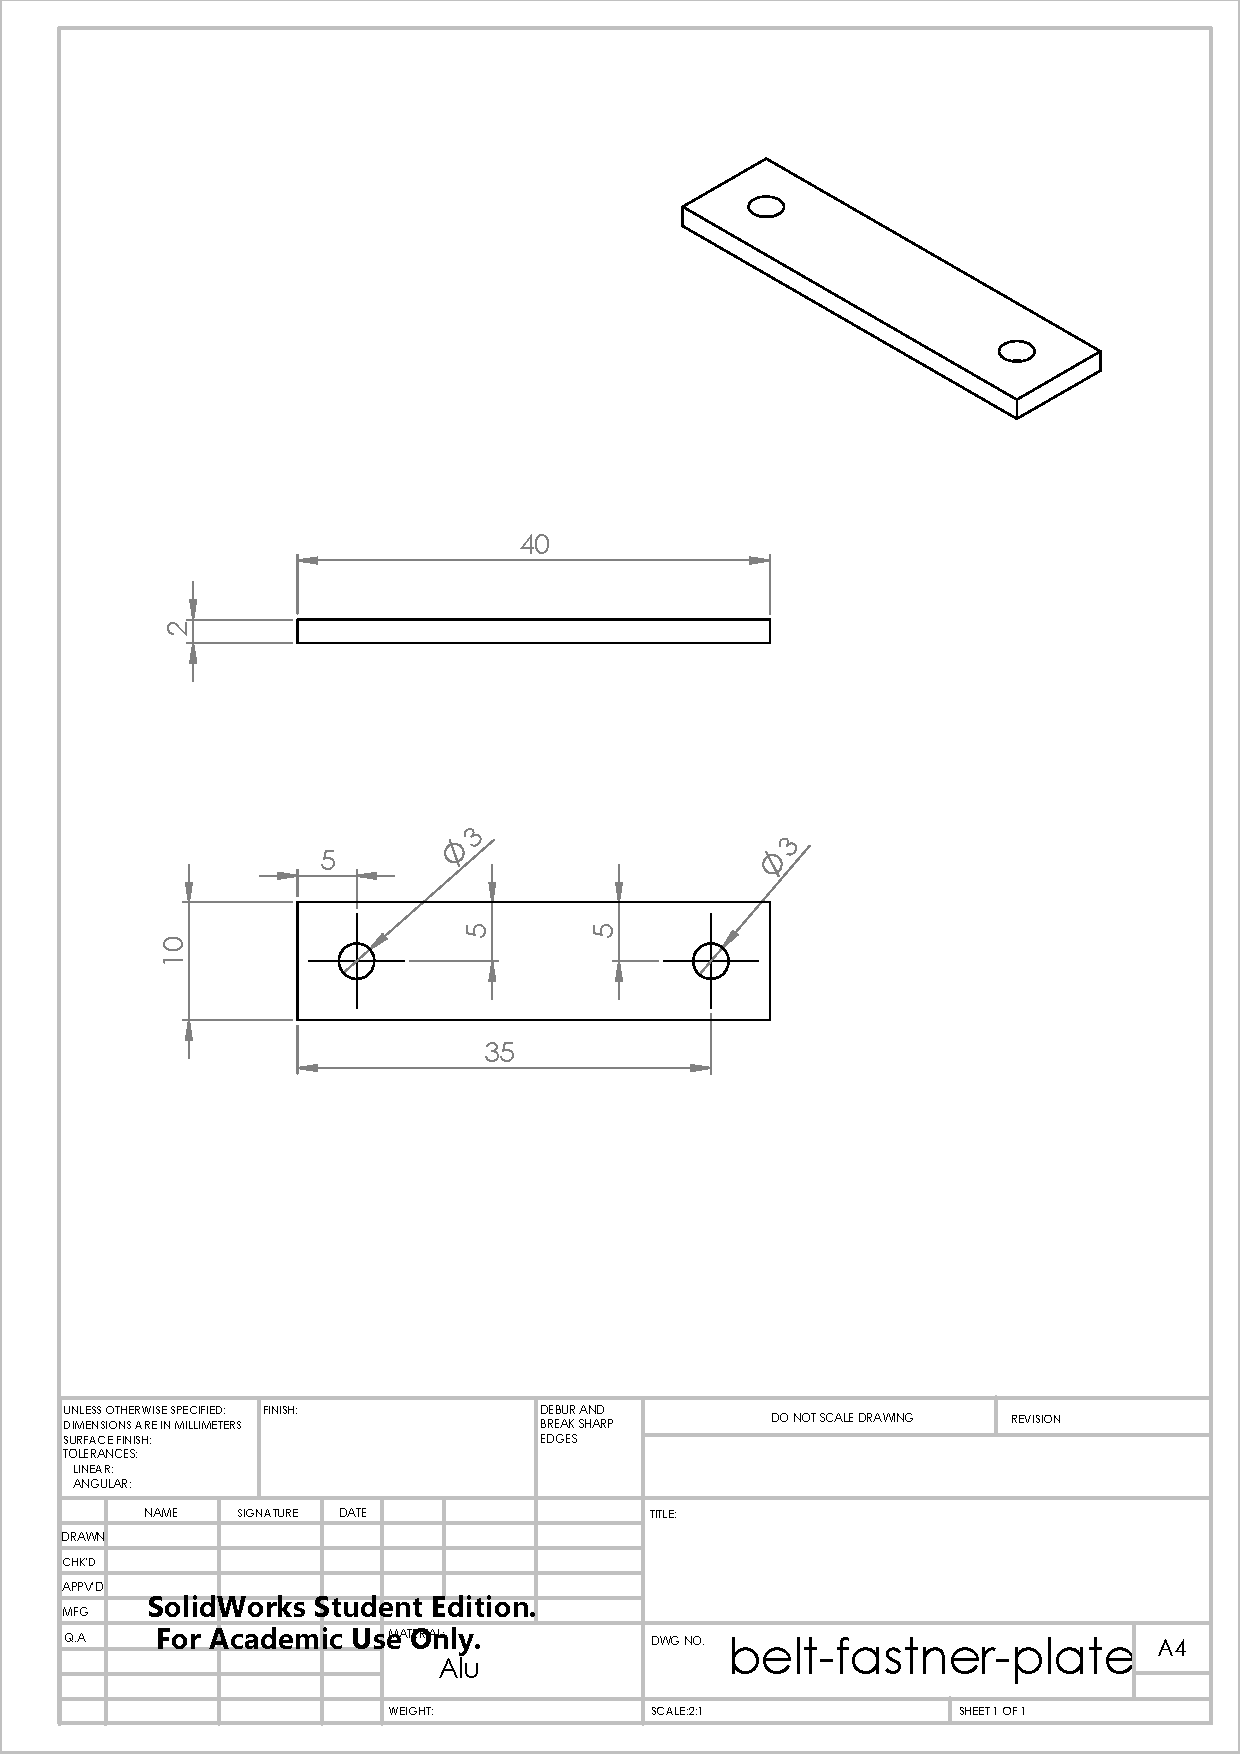
\includepdf[pages={-}]{graphics/cad/belt-fastner-plate.pdf}
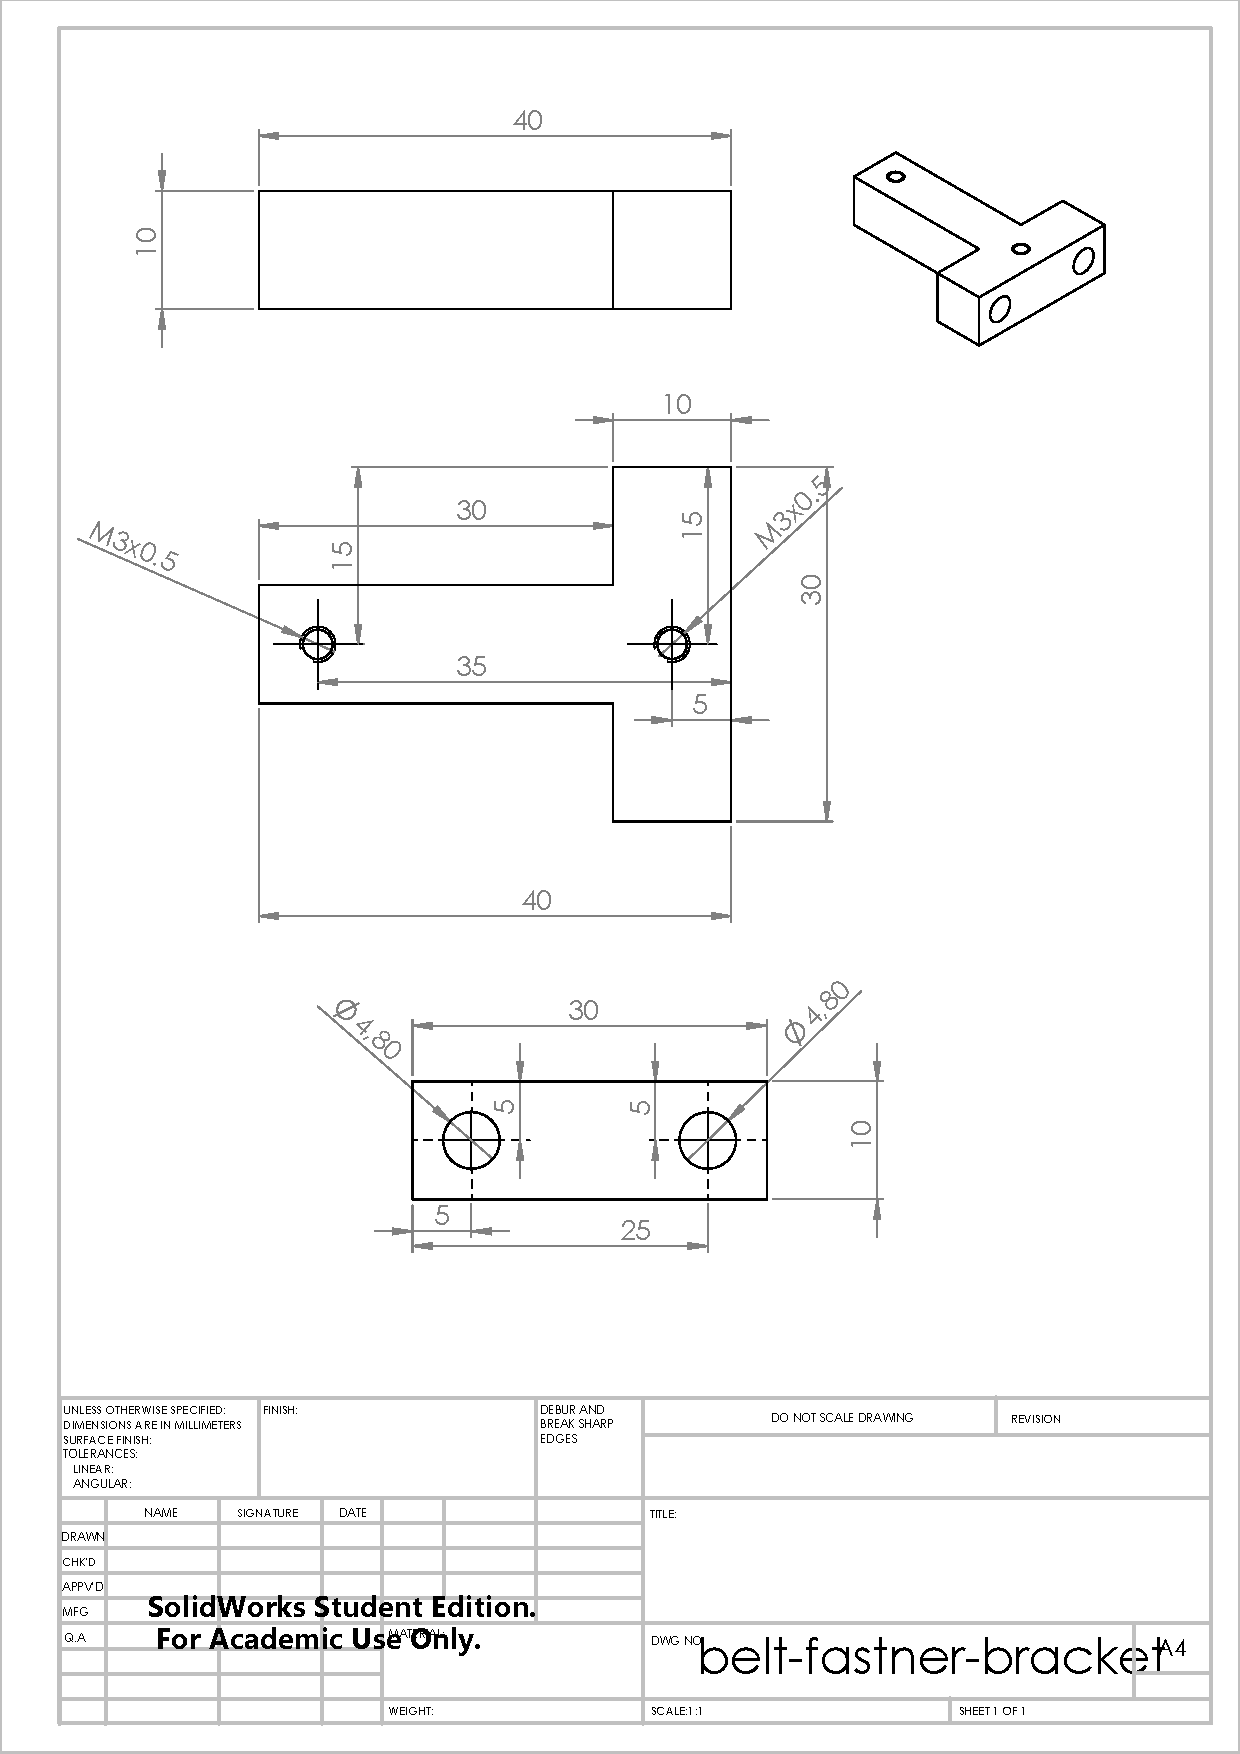
\includepdf[pages={-}]{graphics/cad/belt-fastner-bracket.pdf}
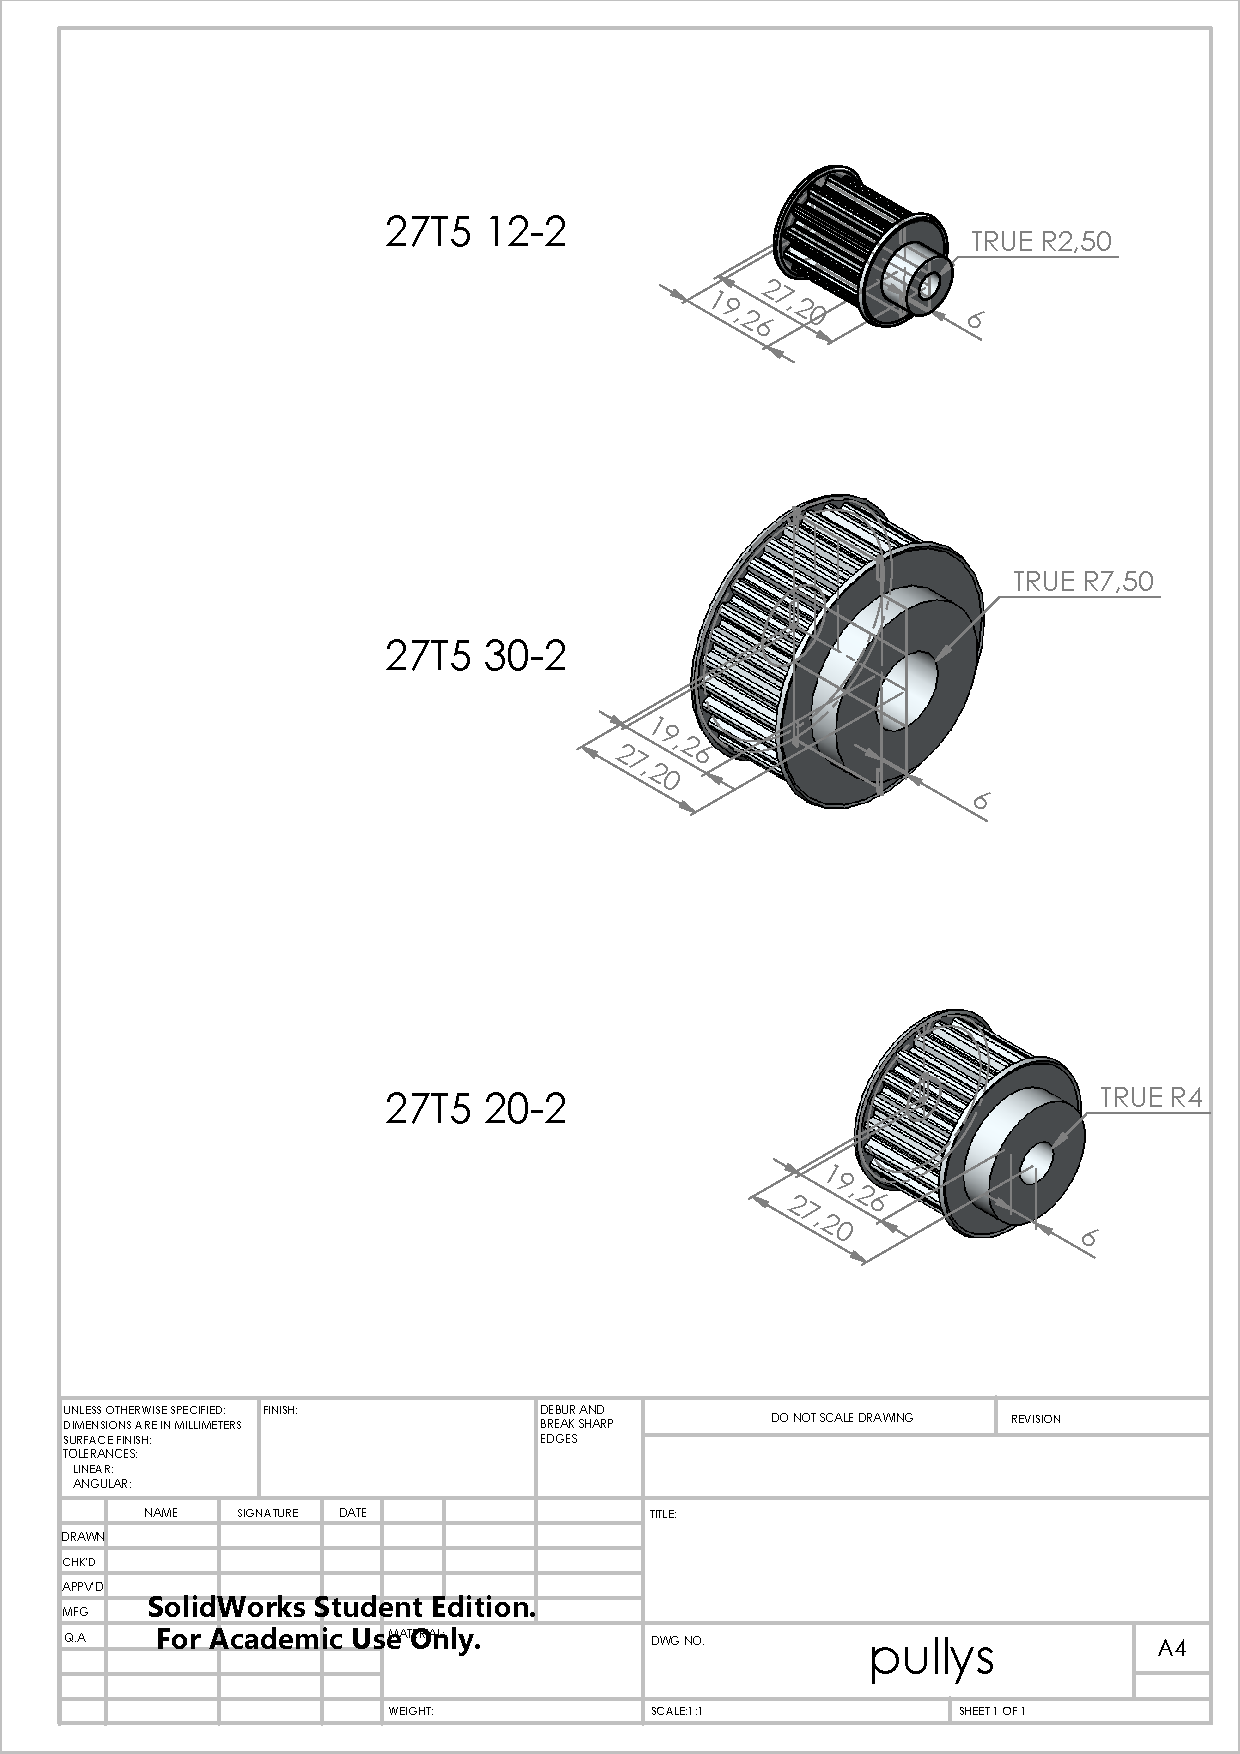
\includepdf[pages={-}]{graphics/cad/pullys.pdf}
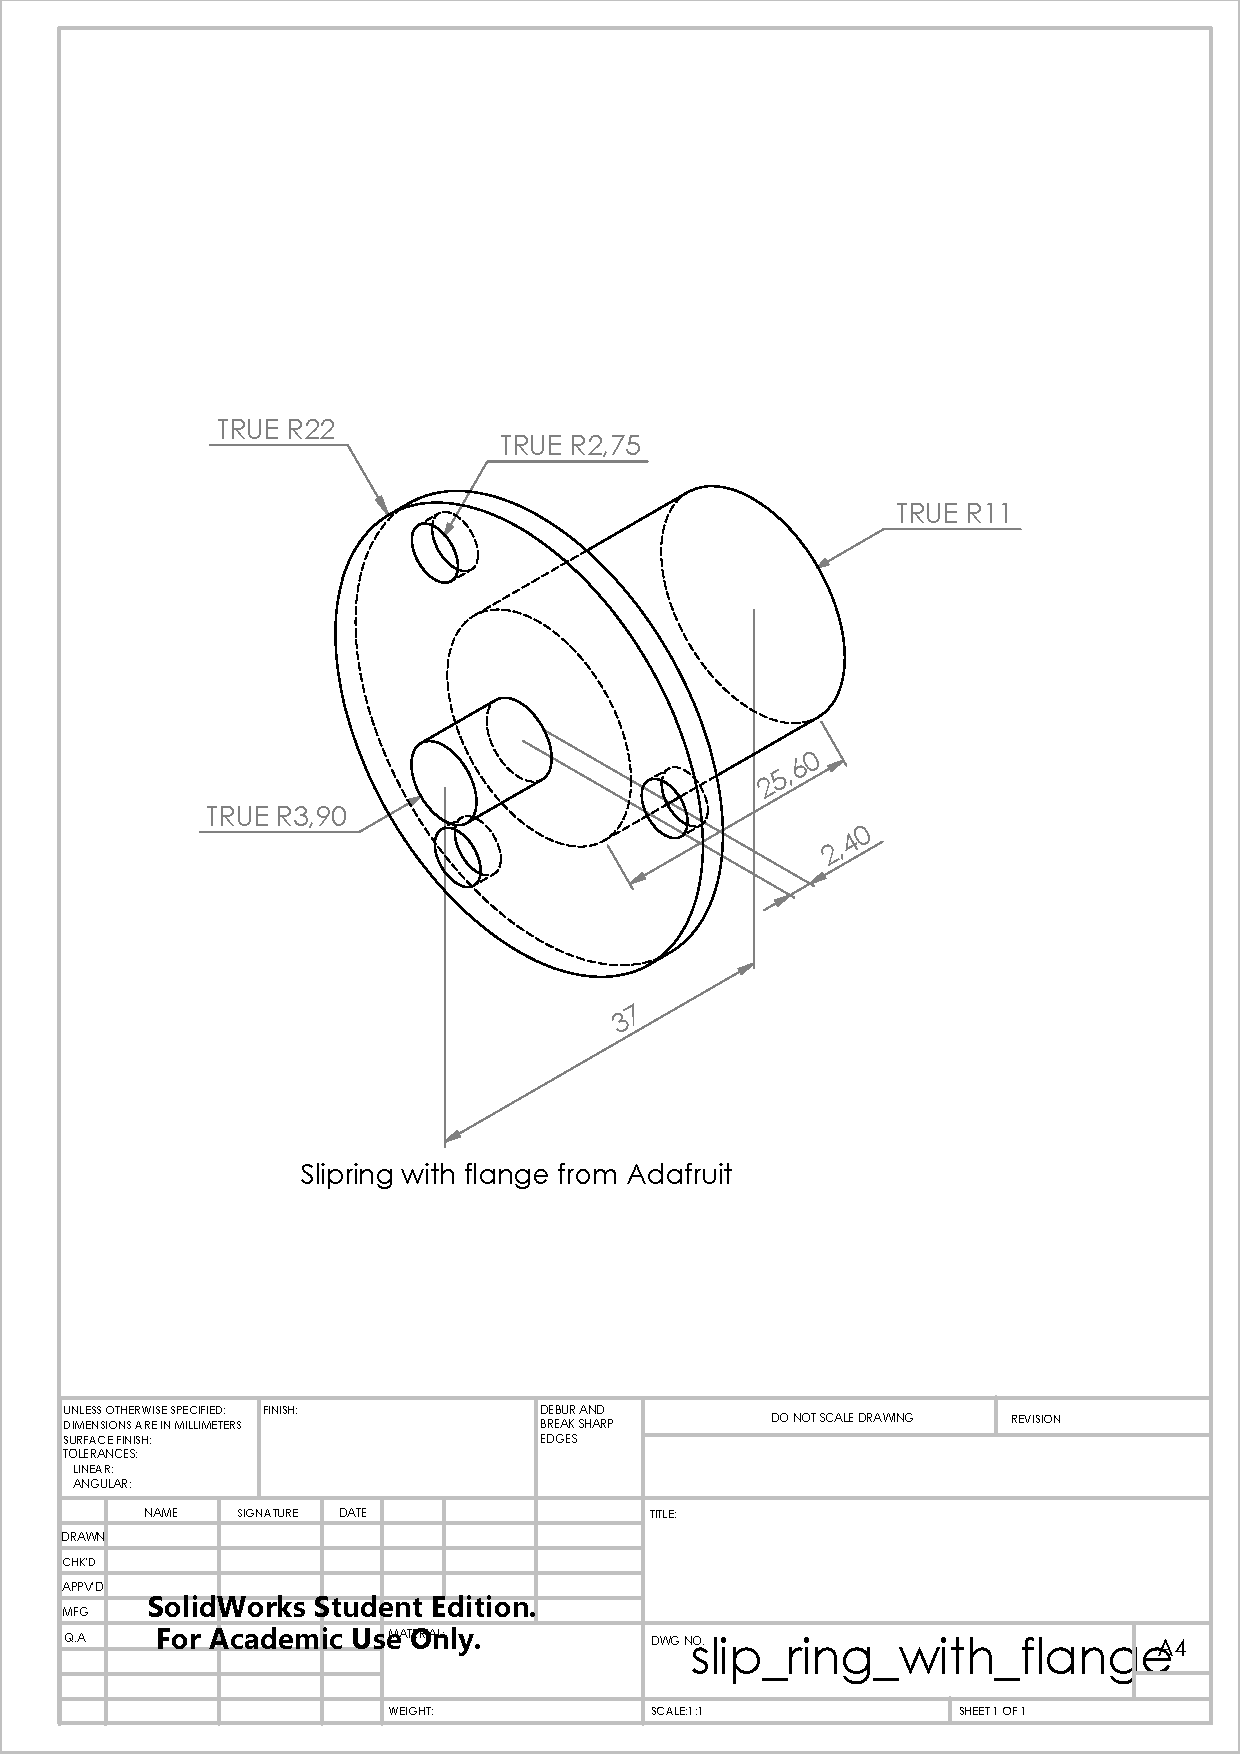
\includepdf[pages={-}]{graphics/cad/slip_ring_with_flange.pdf}

\subsection{Helipad}
The Helipad is the platform where the UAV land and take off. In the middle of the platform a hole for the cable is made. Next to this hole two counterbore holes fits to mount the horizontal measurement device underneath.

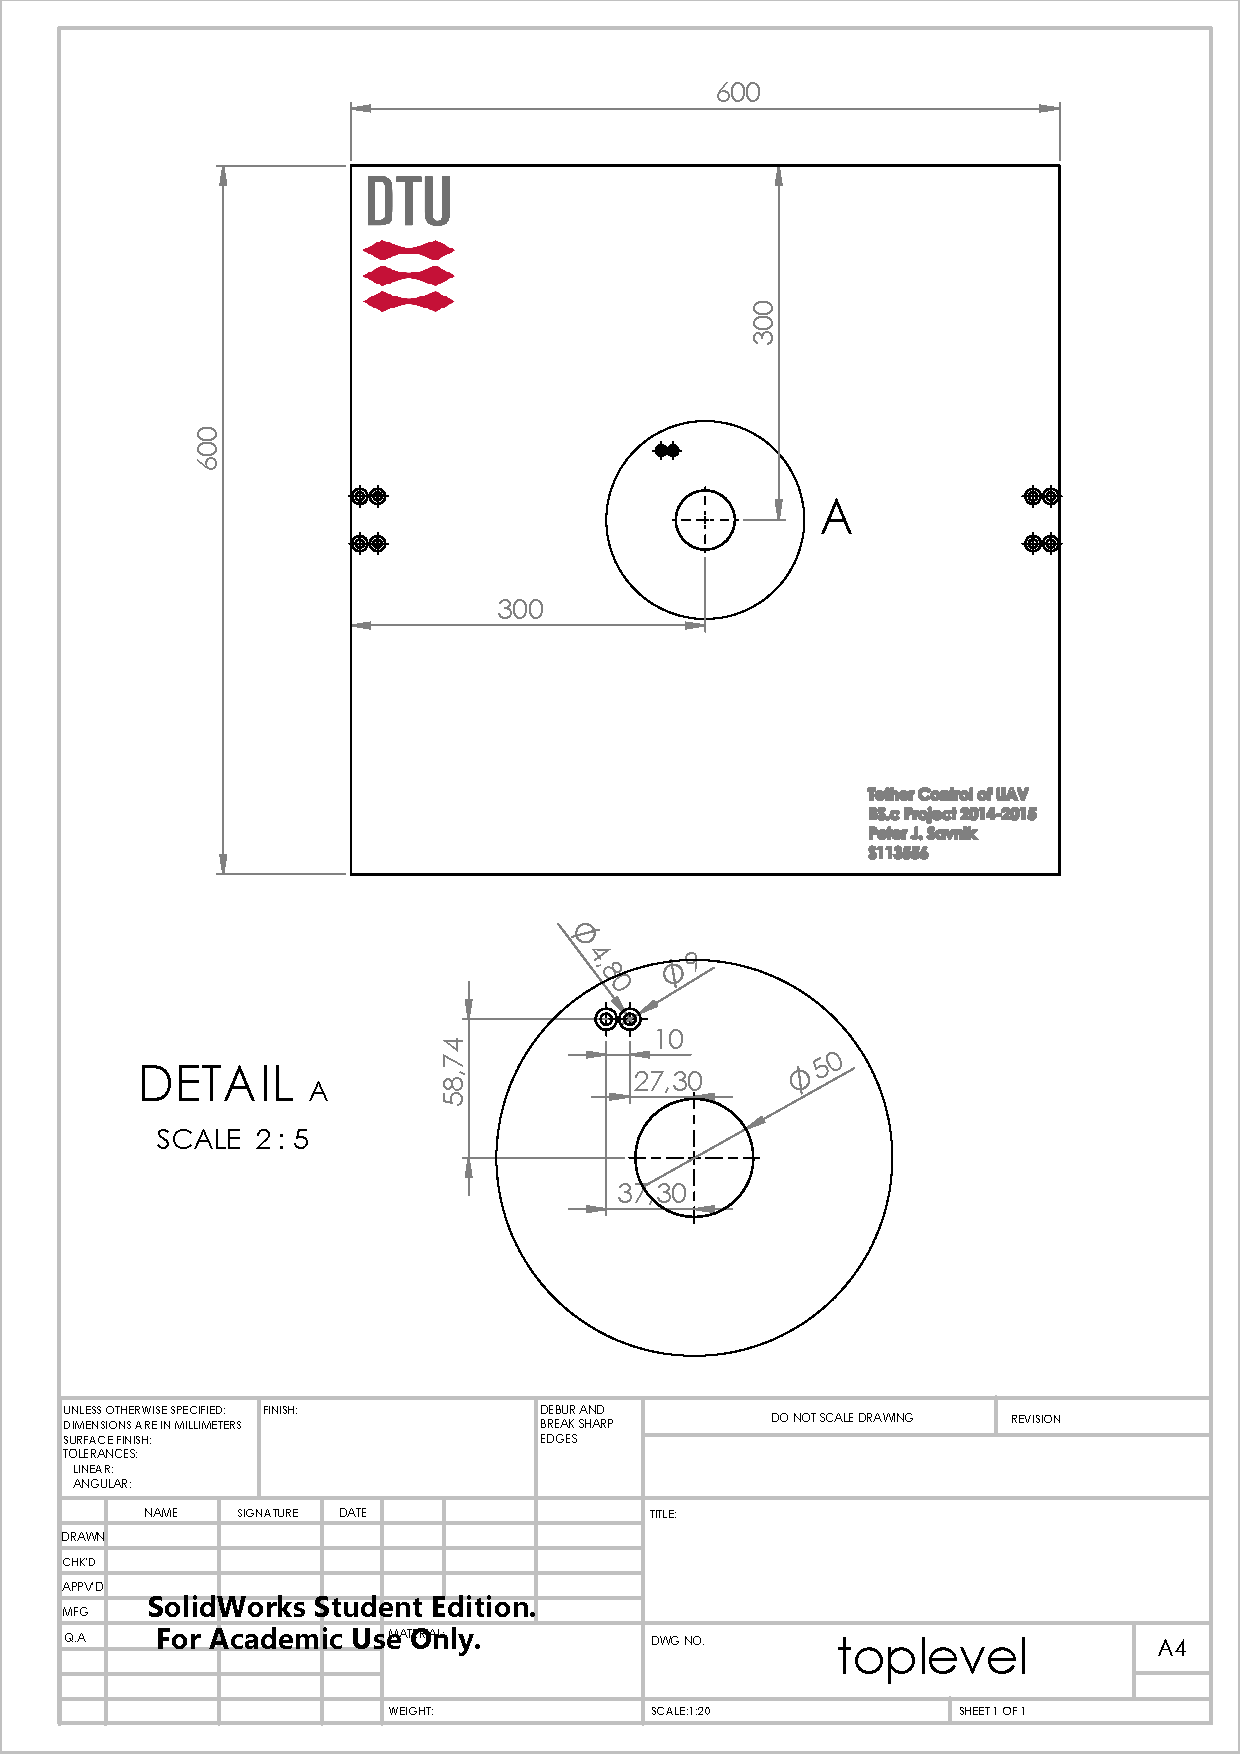
\includepdf[pages={-}]{graphics/cad/toplevel.pdf}

\section{UAV}

The mechanical configuration on the UAV was partially made from a previous project, but was rebuild to fit a Neutrix powercon true connector and slightly adjusted in the configuration height.

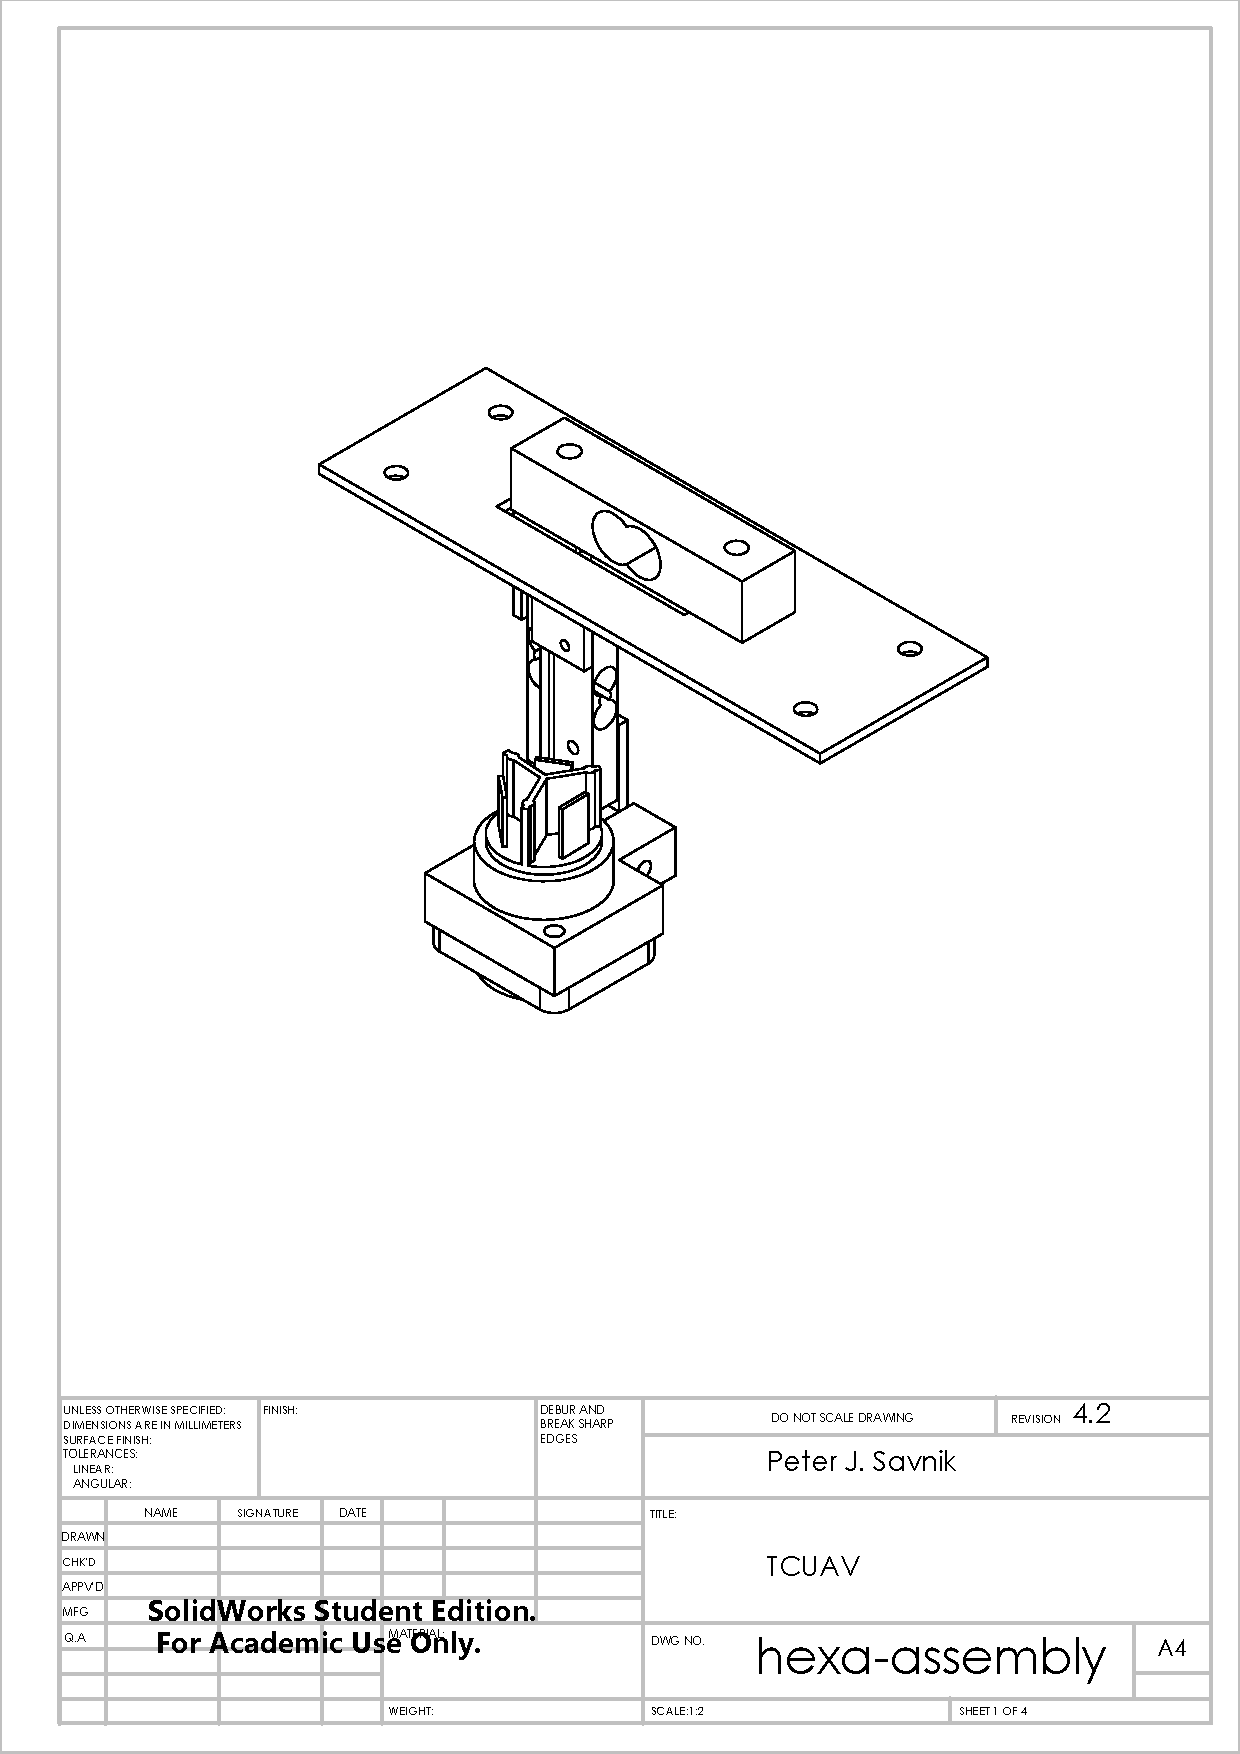
\includepdf[pages={-}]{graphics/cad/hexa-assembly.pdf}
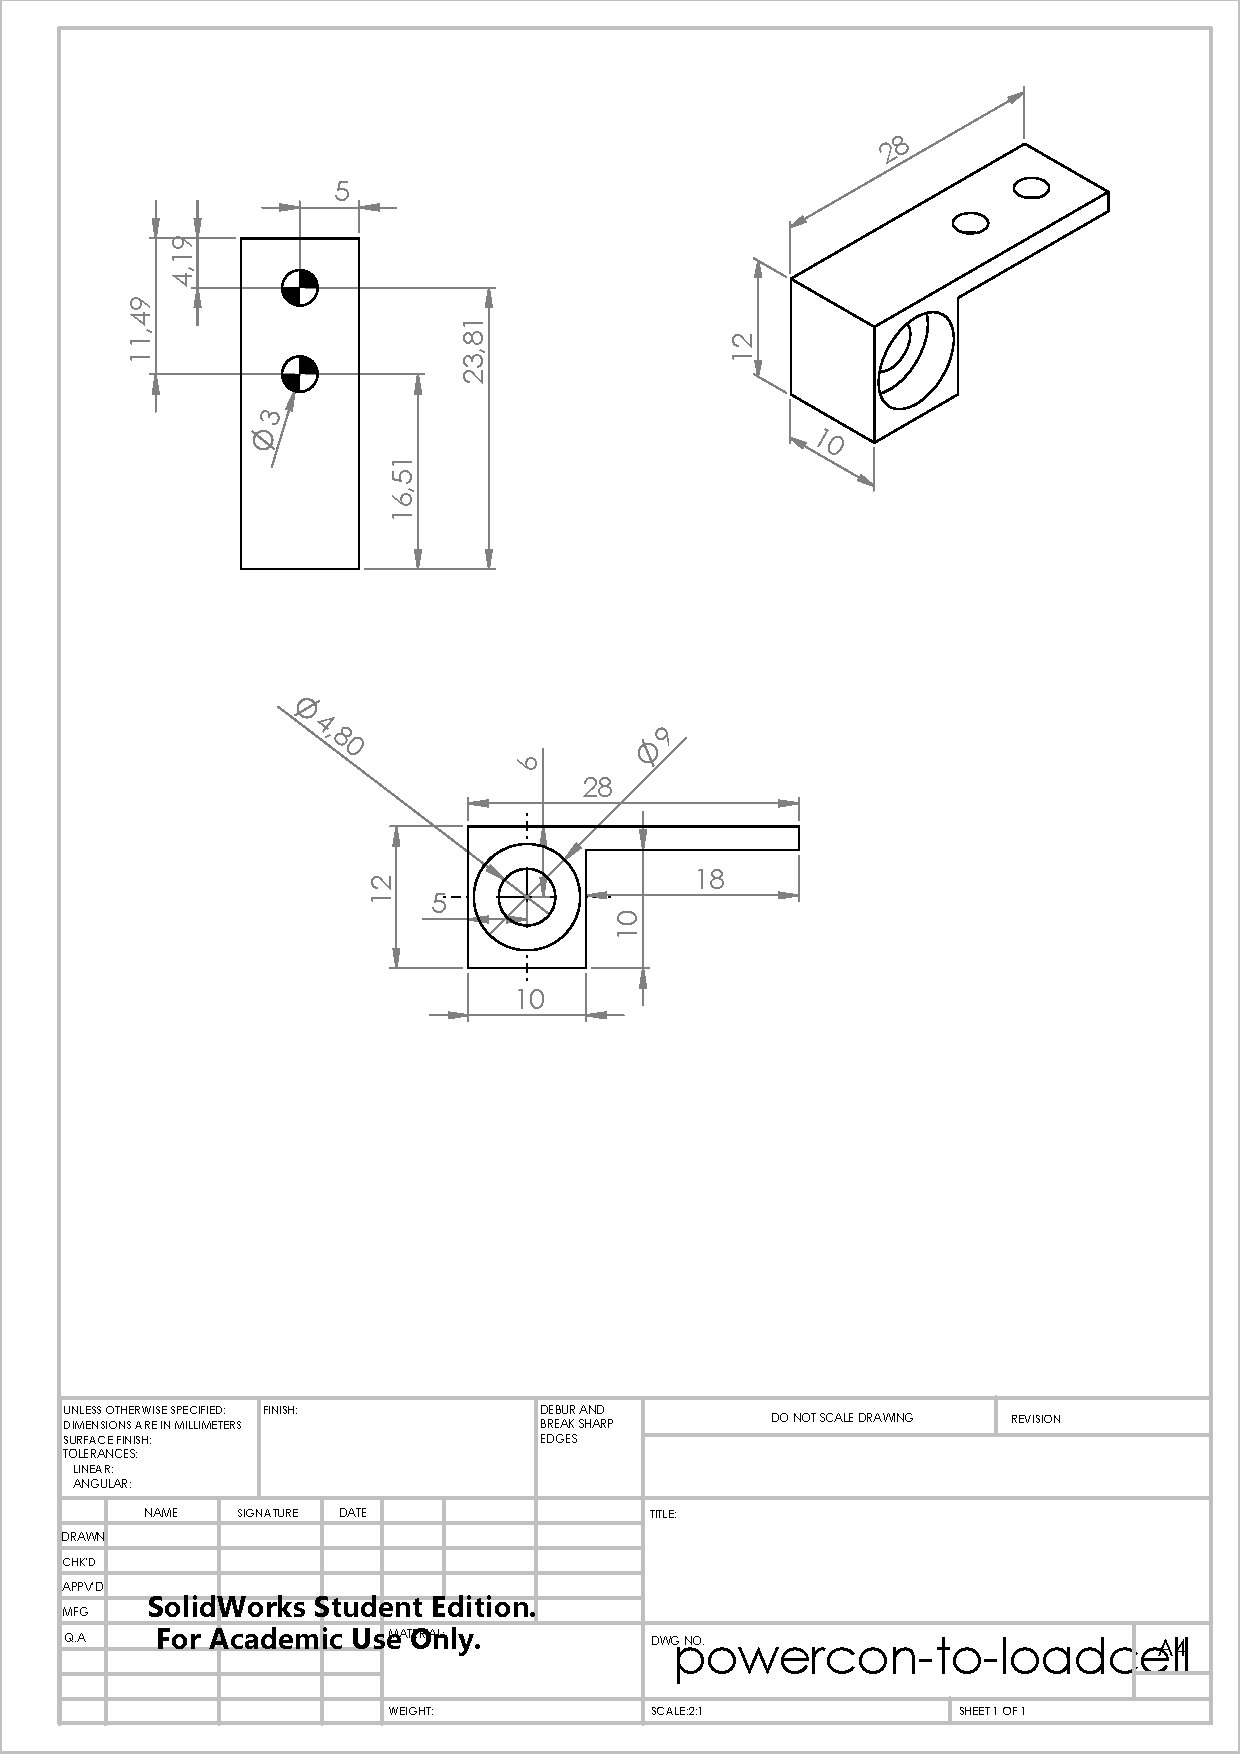
\includepdf[pages={-}]{graphics/cad/powercon-to-loadcell.pdf}
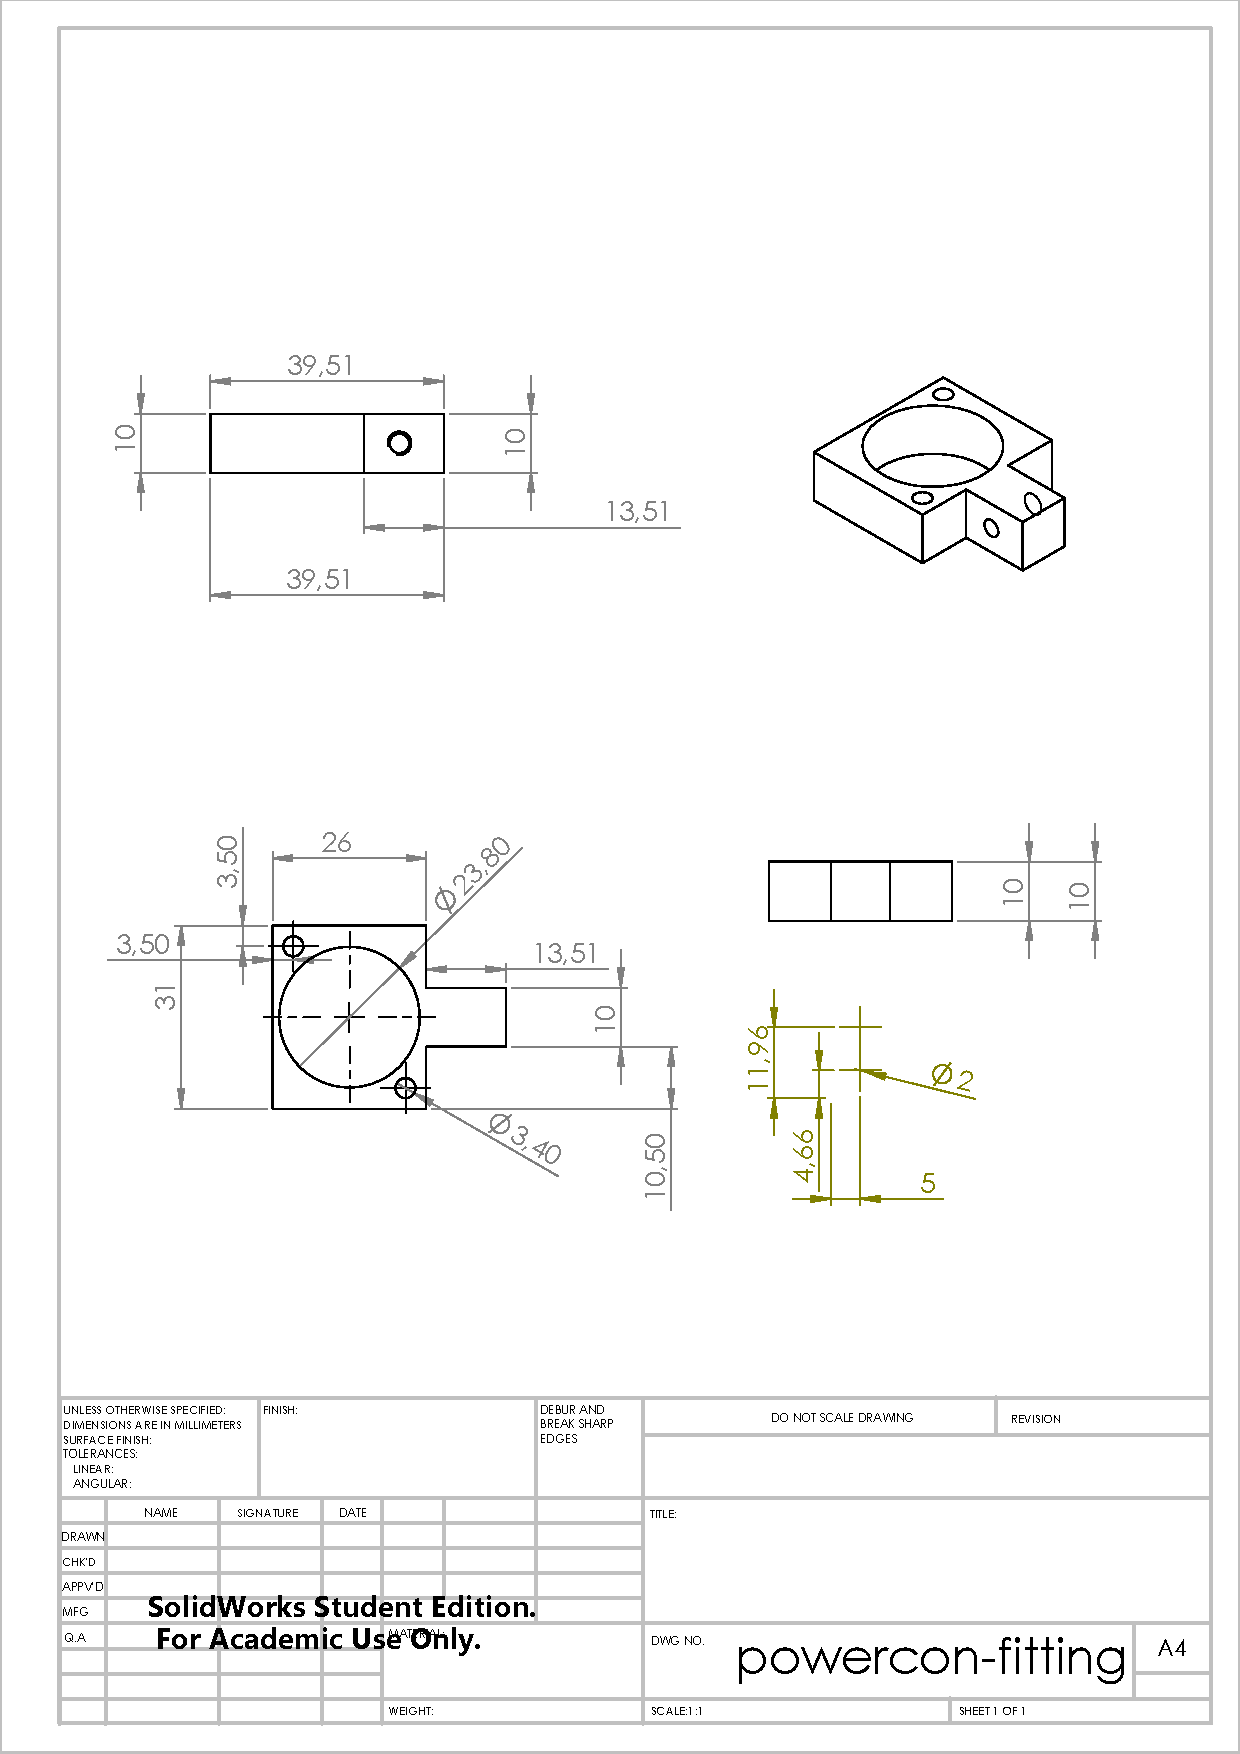
\includepdf[pages={-}]{graphics/cad/powercon-fitting.pdf}
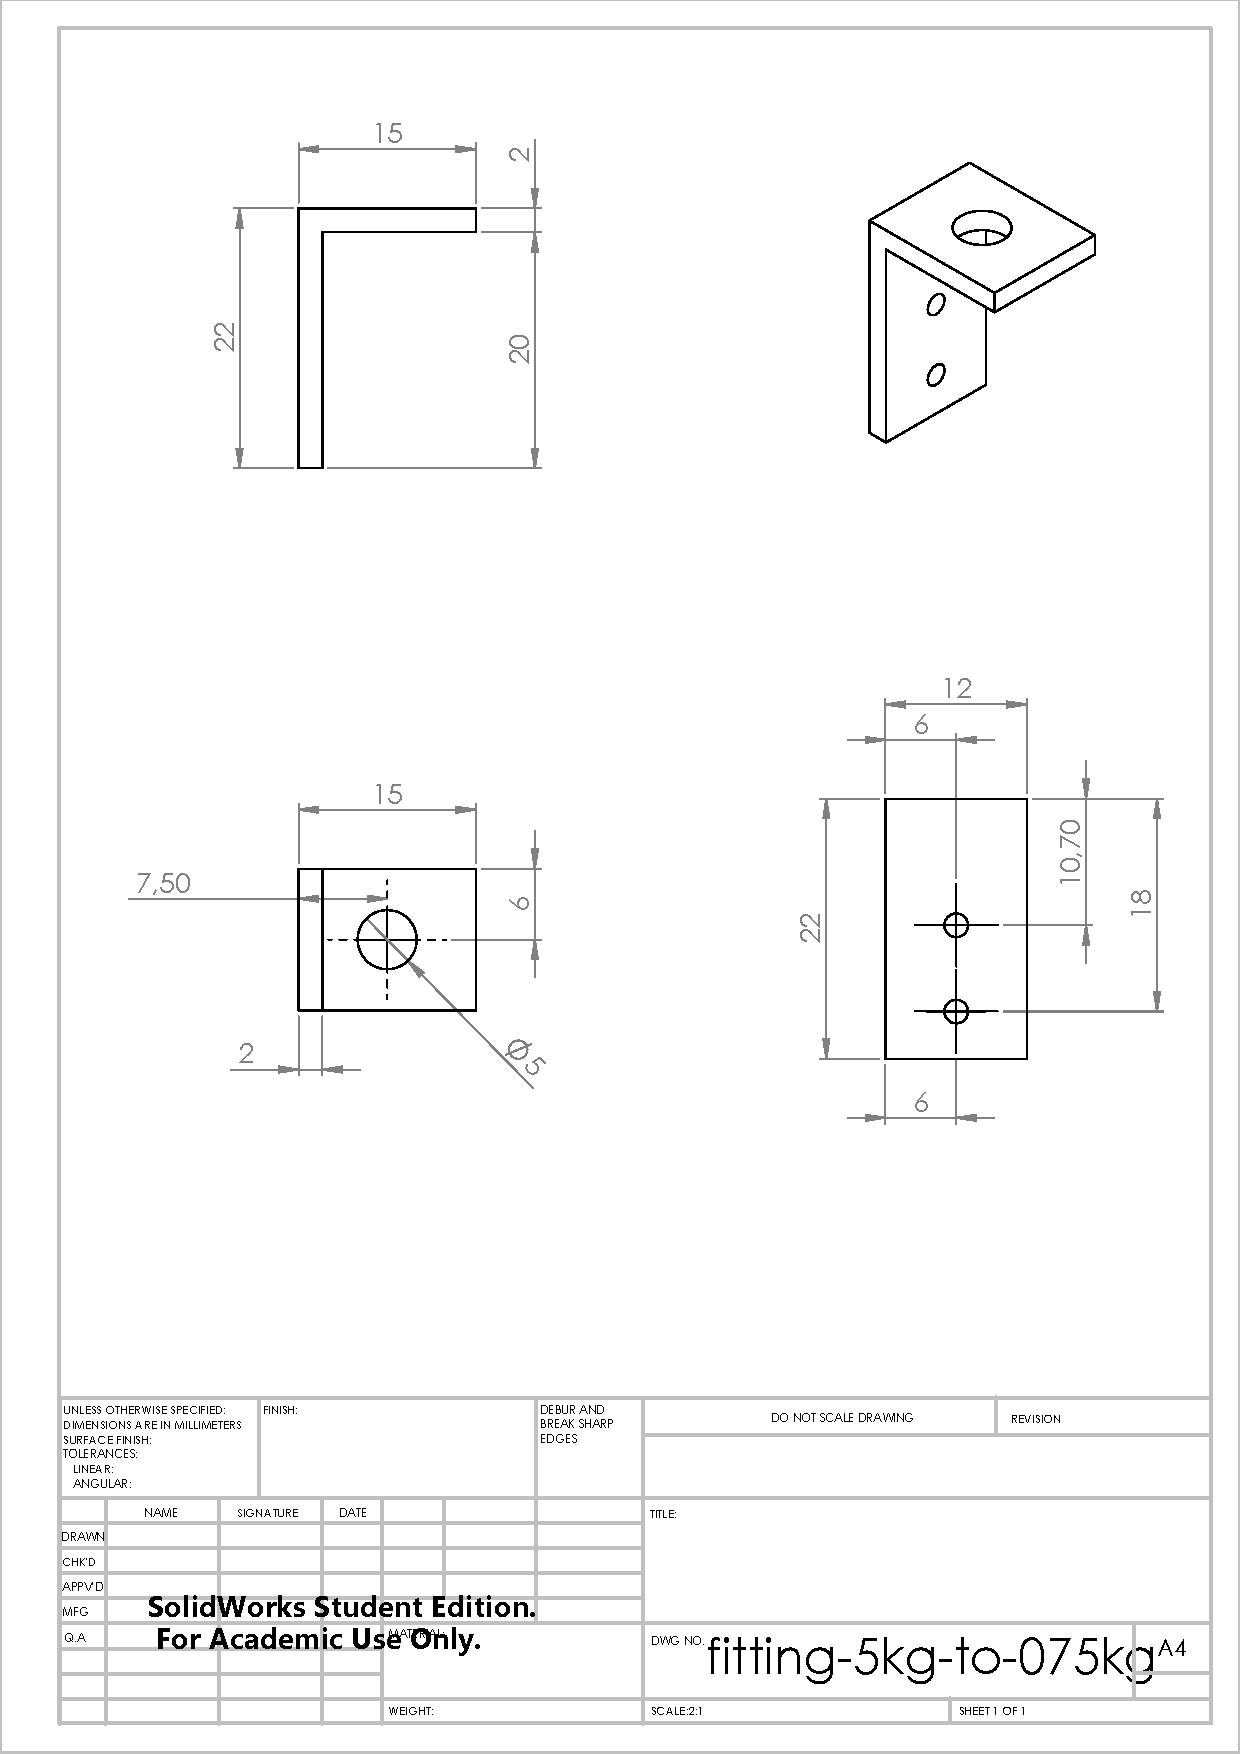
\includepdf[pages={-}]{graphics/cad/fitting-5kg-to-075kg.pdf}
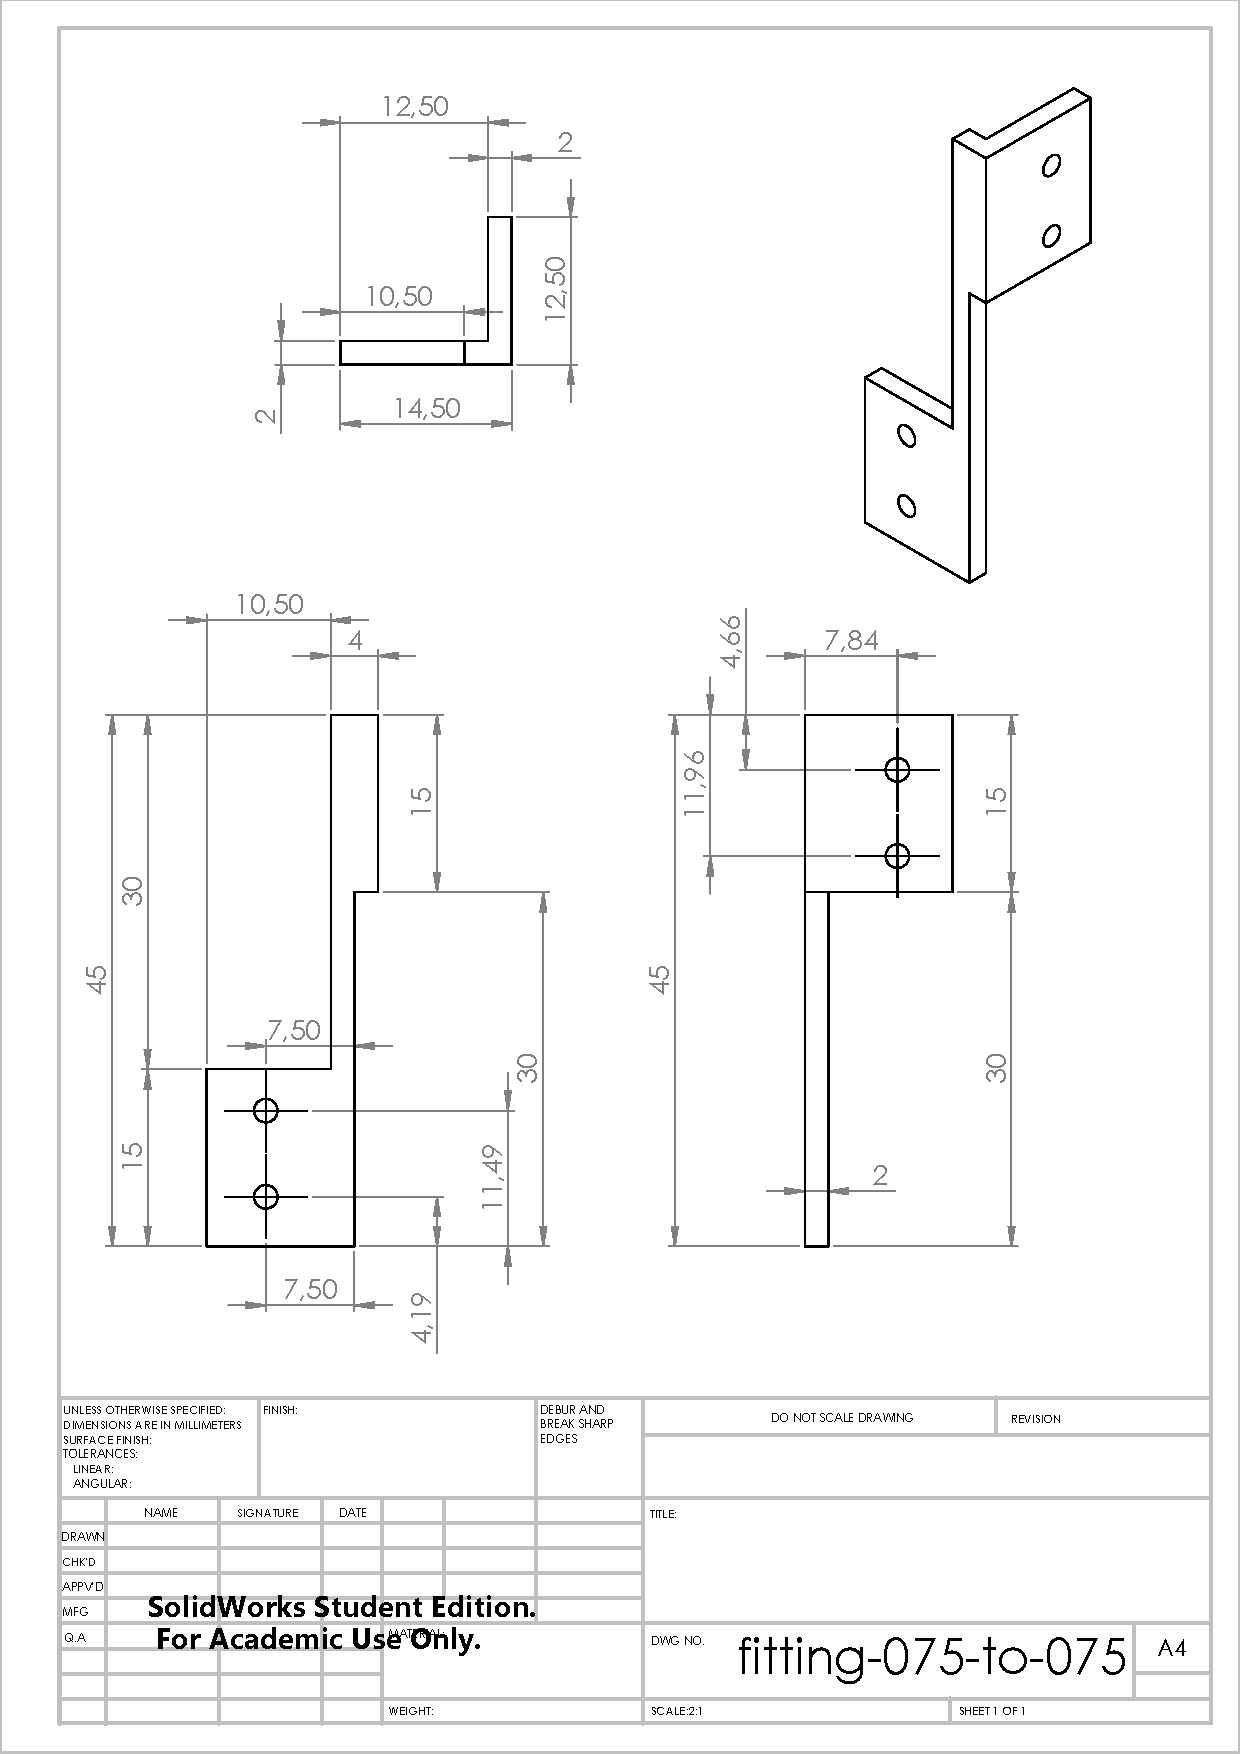
\includepdf[pages={-}]{graphics/cad/fitting-075-to-075.pdf}
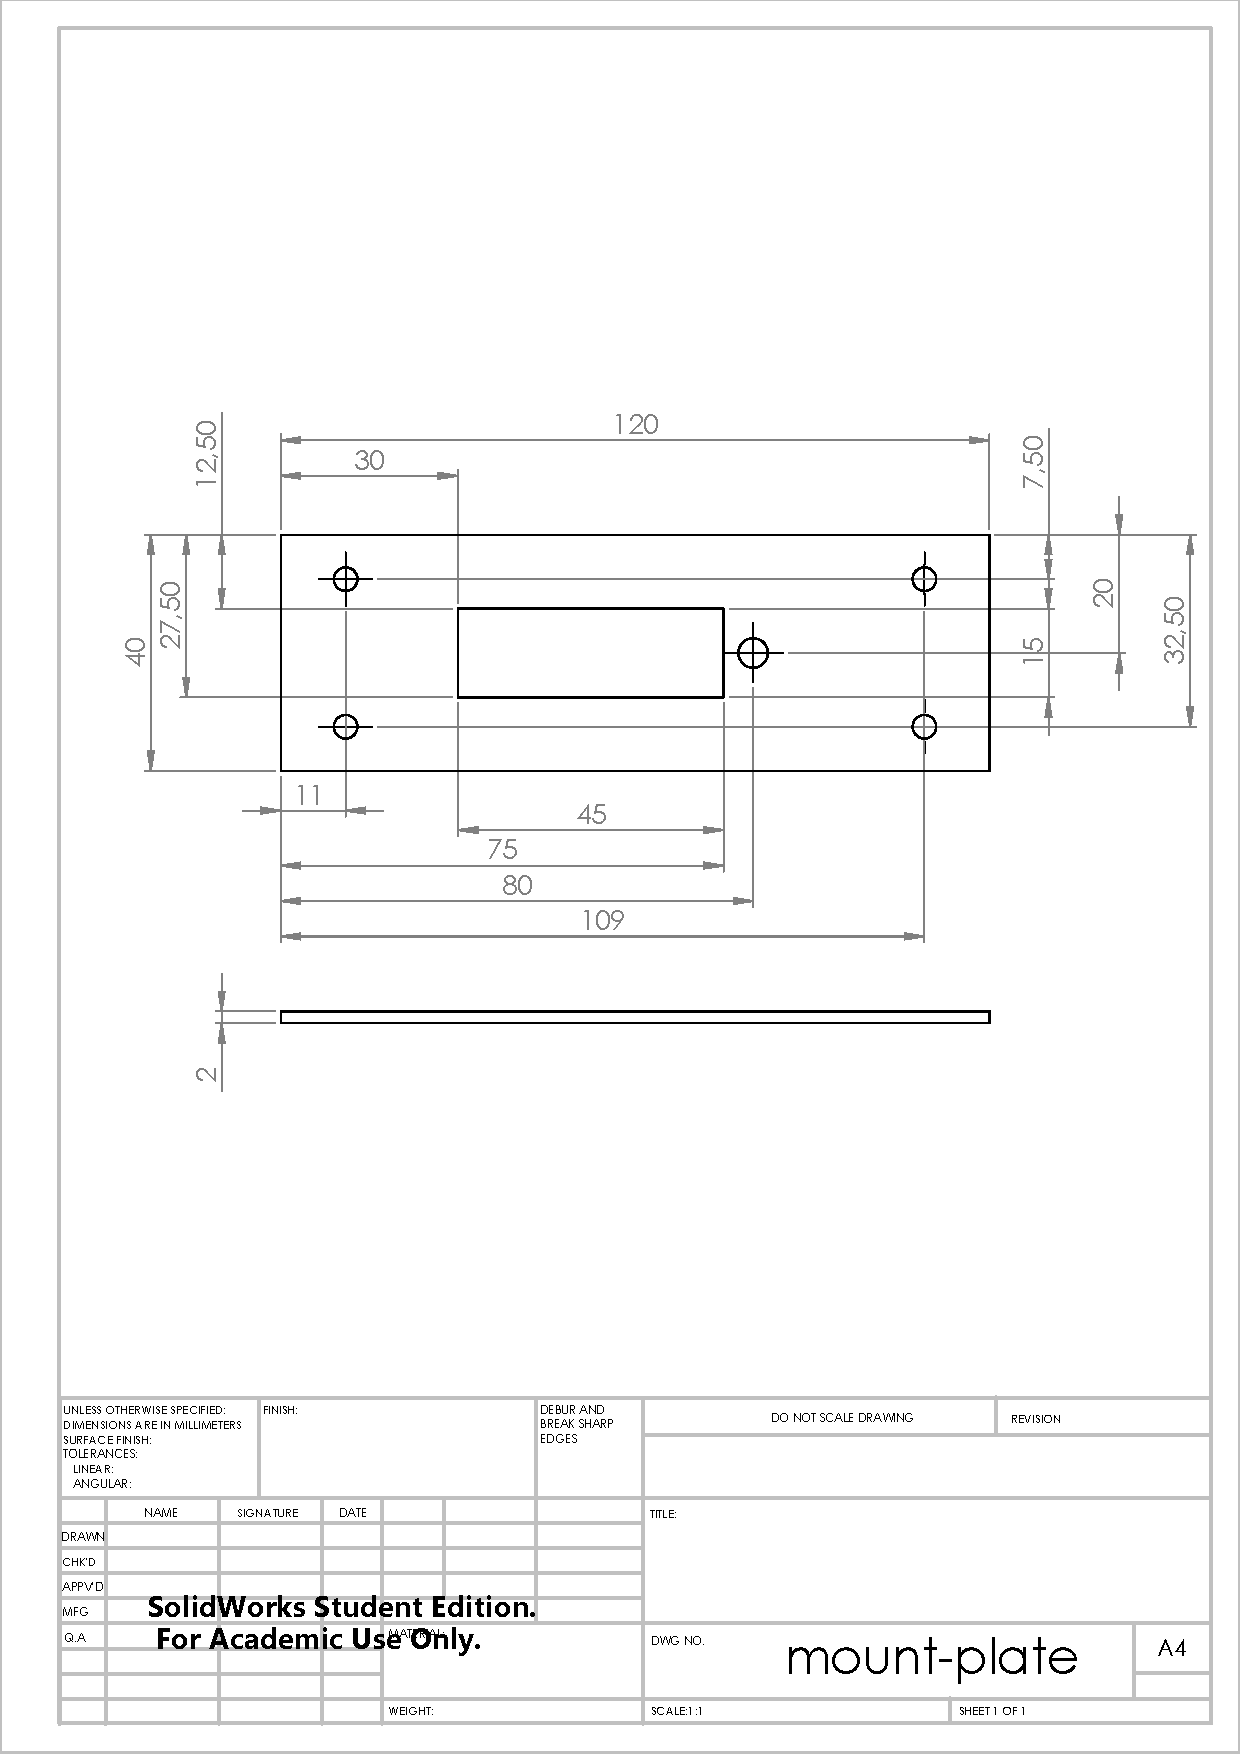
\includepdf[pages={-}]{graphics/cad/mount-plate.pdf}


